\section{Evaluation} \label{sec-evaluation} 
In this section, we evaluate the performance of our collaborative optimizer.
We first describe the setup of the experiment.
Then, we show the end-to-end run-time improvement of our optimizer.
Finally, we investigate the effect of the individual contributions, i.e., materialization and reuse algorithms, on the run-time and storage cost.
\begin{table*}[ht]
\begin{tabular}{lp{0.84\textwidth}rr}
\hline
\textbf{$ID$} & \textbf{$Description$}& \textbf{$N$}& \textbf{$S$}   \\
\hline
1 &  \parbox[t]{0.84\textwidth}{\linespread{0.5}\selectfont \small A real Kaggle script. It includes several feature engineering operations before training logistic regression, random forest, and gradient boosted tree models \cite{start-here-a-gentle-intro}.} & 397 & 14.5\\[0.4cm]

2 &   \parbox[t]{0.84\textwidth}{\linespread{0.5}\selectfont \small A real Kaggle script. It joins multiple datasets, preprocesses the datasets to generate features, and trains gradient boosted tree models on the generated features \cite{introduction-to-manual-feature-engineering}.} & 406 & 25\\[0.4cm]

3 &   \parbox[t]{0.84\textwidth}{\linespread{0.5}\selectfont \small A real Kaggle script. It is similar to Workload 2, with the resulting preprocessed datasets having more features \cite{introduction-to-manual-feature-engineering-p2}.} & 146 & 83.5\\[0.4cm]

4 & \parbox[t]{0.84\textwidth}{\linespread{0.5}\selectfont \small A real Kaggle script that modifies Workload 1 and trains a gradient boosted tree with a different set of hyperparameters \cite{start-here-a-gentle-intro-carlos}.} & 280 & 10\\[0.4cm]

5 & \parbox[t]{0.84\textwidth}{\linespread{0.5}\selectfont \small A real Kaggle script that modifies Workload 1 and performs random and grid search for gradient boosted tree model using generated features of Workload 1 \cite{begining-with-lightgbm-in-detail}.} & 402 & 13.8\\[0.4cm]

6 & \parbox[t]{0.84\textwidth}{\linespread{0.5}\selectfont \small A custom script based on Workloads 2 and 4. It trains a gradient boosted tree on the generated features of Workload 2.} & 121 & 21\\[0.15cm]

7 & \parbox[t]{0.84\textwidth}{\linespread{0.5}\selectfont \small A custom script based on Workload 3 and 4. It trains a gradient boosted tree on the generated features of Workload 3.} & 145 & 83\\[0.15cm]

8 & \parbox[t]{0.84\textwidth}{\linespread{0.5}\selectfont \small A custom script that joins the features of Workloads 1 and 2. Then, similar to Workload 4, it trains a gradient boosted tree on the joined dataset.} & 341 & 21.1\\
\hline
\end{tabular}
\caption{Description of Kaggle workloads. $N$ is number of the artifacts and $S$ is the total size of the artifacts in GB.}
\label{kaggle-workload}
\vspace{-4mm}
\end{table*}
\subsection{Setup}
We execute the experiments on a Linux Ubuntu machine with 128 GB of RAM.
We implement a prototype of our system in python 2.7.12.
We implement EG using NetworkX 2.2 \cite{hagberg2008exploring}.
We run every experiment 3 times and report the average.

\textbf{Baseline and other System.}
We compare our system with a naive baseline, i.e., executing all the workloads without any optimization, and Helix \cite{xin2018helix}.
Helix is a system for optimizing ML workloads, where users \textit{iterate} on workloads by testing out small modifications until achieving the desired solution.
Helix utilizes materialization and reuse of the intermediate artifacts to speed up the execution of ML workloads within a single session.
Helix materializes an artifact when its recreation cost is greater than twice its load cost (Algorithm 2 of the Helix paper \cite{xin2018helix}).
To find the optimal reuse plan, Helix reduces the workload DAG into an instance of the project selection problem (PSP) and solve it via the Max-Flow algorithm \cite{algodesign}.
In our implementation of Helix reuse, we consulted the authors and followed Algorithm 1 of the Helix paper to transform the workload DAG into PSP.
Similar to Helix, we utilized the Edmonds-Karp Max-Flow algorithm \cite{edmonds1972theoretical}, which runs in polynomial time ($\mathcal{O}(|V|.|E|^2)$).

\textbf{Kaggle workloads.} 
In the Kaggle workloads, we recreate the use case in Section \ref{sec-background}.
We use eight workloads, which generate 130 GB of artifacts.
There are five real and three custom workloads.
Table \ref{kaggle-workload} shows details of the workloads.
There are 9 source datasets with a total size of 2.5 GB.
Unless specified otherwise, we use storage-aware materialization with a budget of 16 GB and $\alpha=0.5$.
For Helix, we also set the materialization budget to 16 GB.

\textbf{OpenML workloads.} 
In the OpenML workloads, we extracted 2000 runs of scikit-learn pipelines for Task 31 from the OpenML platform \cite{openml-31}.
The dataset is small, and the total size of the artifacts after executing the 2000 runs is 1.5 GB.
We use the OpenML workloads to show the effects of the model quality on materialization and model warmstarting on run-time.
Unless specified otherwise, we use storage-aware materialization with a budget of 100 MB and $\alpha=0.5$.

\subsection{End-to-end Optimization}
In this experiment, we evaluate the impact of our optimizer on the Kaggle workloads.
In our motivating example, we describe three workloads (Workloads 1-3 of Table \ref{kaggle-workload}), that are copied and modified 7,000 times by different users.
Therefore, at the very least, users execute these workloads 7000 times.
\begin{figure}[ht]
\centering
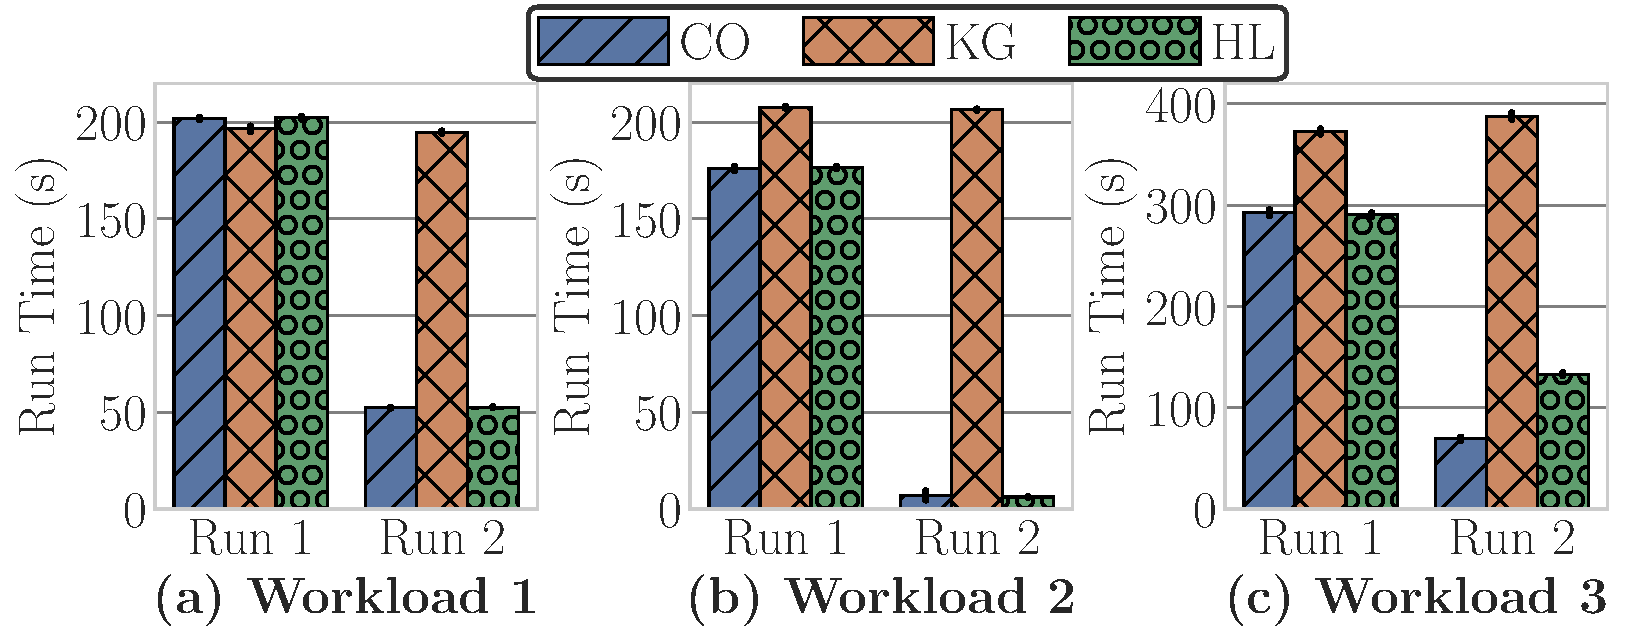
\includegraphics[width=1.0\columnwidth]{images/experiment-results/kaggle_home_credit/execution_time/repeated_workloads}
\caption{Repeated executions of Kaggle workloads}
\label{exp-execution-repeated-kaggle-workload}
\vspace{-4mm}
\end{figure}

Figure \ref{exp-execution-repeated-kaggle-workload} shows the result of repeating the execution of each workload twice.
Before the first run, EG is empty. 
Therefore, the default baseline (KG), Helix (HL), and our collaborative optimizer (CO) must execute all the operations in the workloads.
In Workload 1, the run-time of CO and HL is slightly larger than KG in the first run.
Workload 1 executes two alignment operations.
An alignment operation receives two datasets, removes all the columns that do not appear in both datasets, and returns the resulting two datasets.
In CO, we need to measure the precise compute-cost of every artifact.
This is not possible for operations that return multiple artifacts.
Thus, we re-implemented the alignment operation, which is less optimized than the baseline implementation.
In Workloads 2 and 3, CO and HL outperform KG even in the first run.
Both Workloads 2 and 3 contain many redundant operations.
The local pruning step of our optimizer identifies the redundancies and only execute such operations once.

In the second run of the workloads, CO reduces the run-time by an order of magnitude for Workloads 2 and 3.
Workload 1 executes an external and compute-intensive visualization command that computes a bivariate kernel density estimate.
Since our optimizer does not materialize such external information, it must re-execute the operation; thus, resulting in a smaller run-time reduction.

HL has similar performance to CO in Workloads 1 and 2.
However, CO outperforms HL in Workload 3. 
The total size of the artifacts in Workloads 1 and 2 is small.
As a result, a large number of artifacts for both HL and CO are materialized.
Our reuse algorithm finds the same reuse plan as Helix, therefore, the run-times for Workloads 1 and 2 are similar.
However, the size of the artifacts in Workload 3 is larger than the budget (i.e., 83.5 GB).
The materialization algorithm of HL does not consider the benefit of materializing one artifact over the others and starts materializing the artifacts from the root node until the budget is exhausted.
As a result, many of the high-utility artifacts that appear towards the end of the workloads are not materialized.
The side-effect of the materialization algorithm of HL is visible for Workload 3, where only a handful of the initial artifacts are materialized.
Therefore, HL has to re-execute many of the operations at the end of Workload 3, which results in an overhead of around 70 seconds when compared to CO.
\begin{figure}[t]
\centering
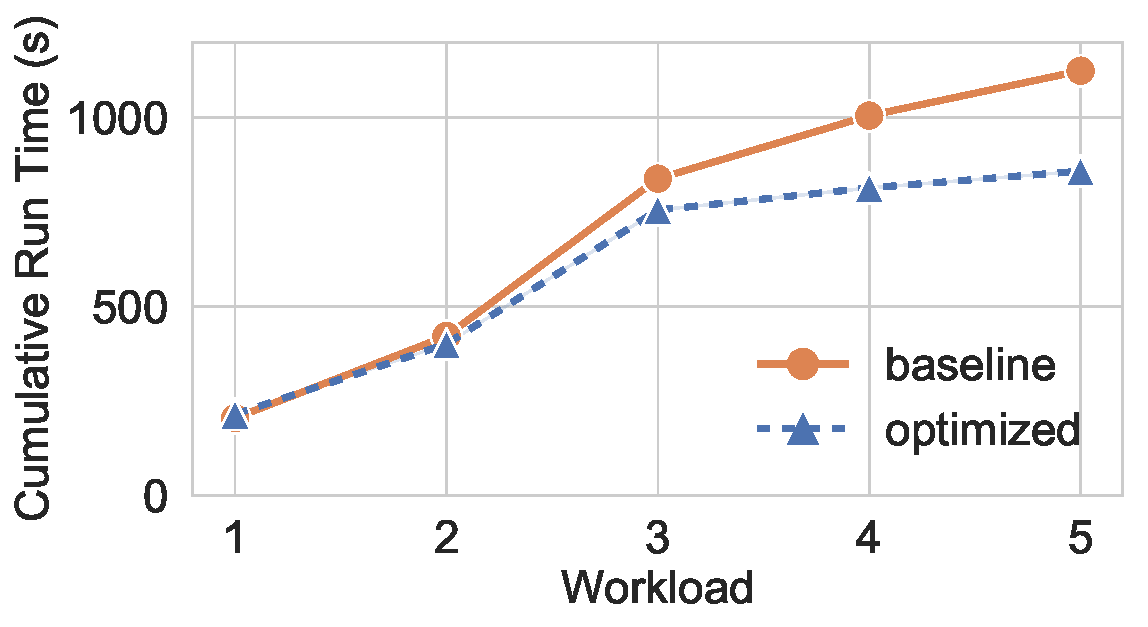
\includegraphics[width=1.0\columnwidth]{images/experiment-results/kaggle_home_credit/execution_time/different_workloads}
\caption{Execution of Kaggle workloads in sequence}
\label{exp-execution-different-kaggle-workload}
\vspace{-4mm}
\end{figure}

Figure \ref{exp-execution-different-kaggle-workload} shows the cumulative run-time of executing the Kaggle workloads consecutively.
Workloads 4-8 operate on the artifacts generated in Workloads 1-3; thus, instead of recomputing those artifacts, CO reuses the artifacts.
As a result, the cumulative run-time of running the 8 workloads decreases by 50\%.
HL also improves run-time when compared to KG. 
However, HL only materializes the initial artifacts of the workloads and has a smaller improvement over KG when compared to CO.

This experiment shows that optimizing a single execution of each workload improves the run-time.
In a real collaborative environment, there are hundreds of modified scripts and possibly thousands of repeated execution of such scripts, resulting in 1000s of hours of improvement in run-time.

\subsection{Materialization}
In this set of experiments, we investigate the impact of different materialization algorithms on storage and run-time.

\begin{figure}[t]
\centering
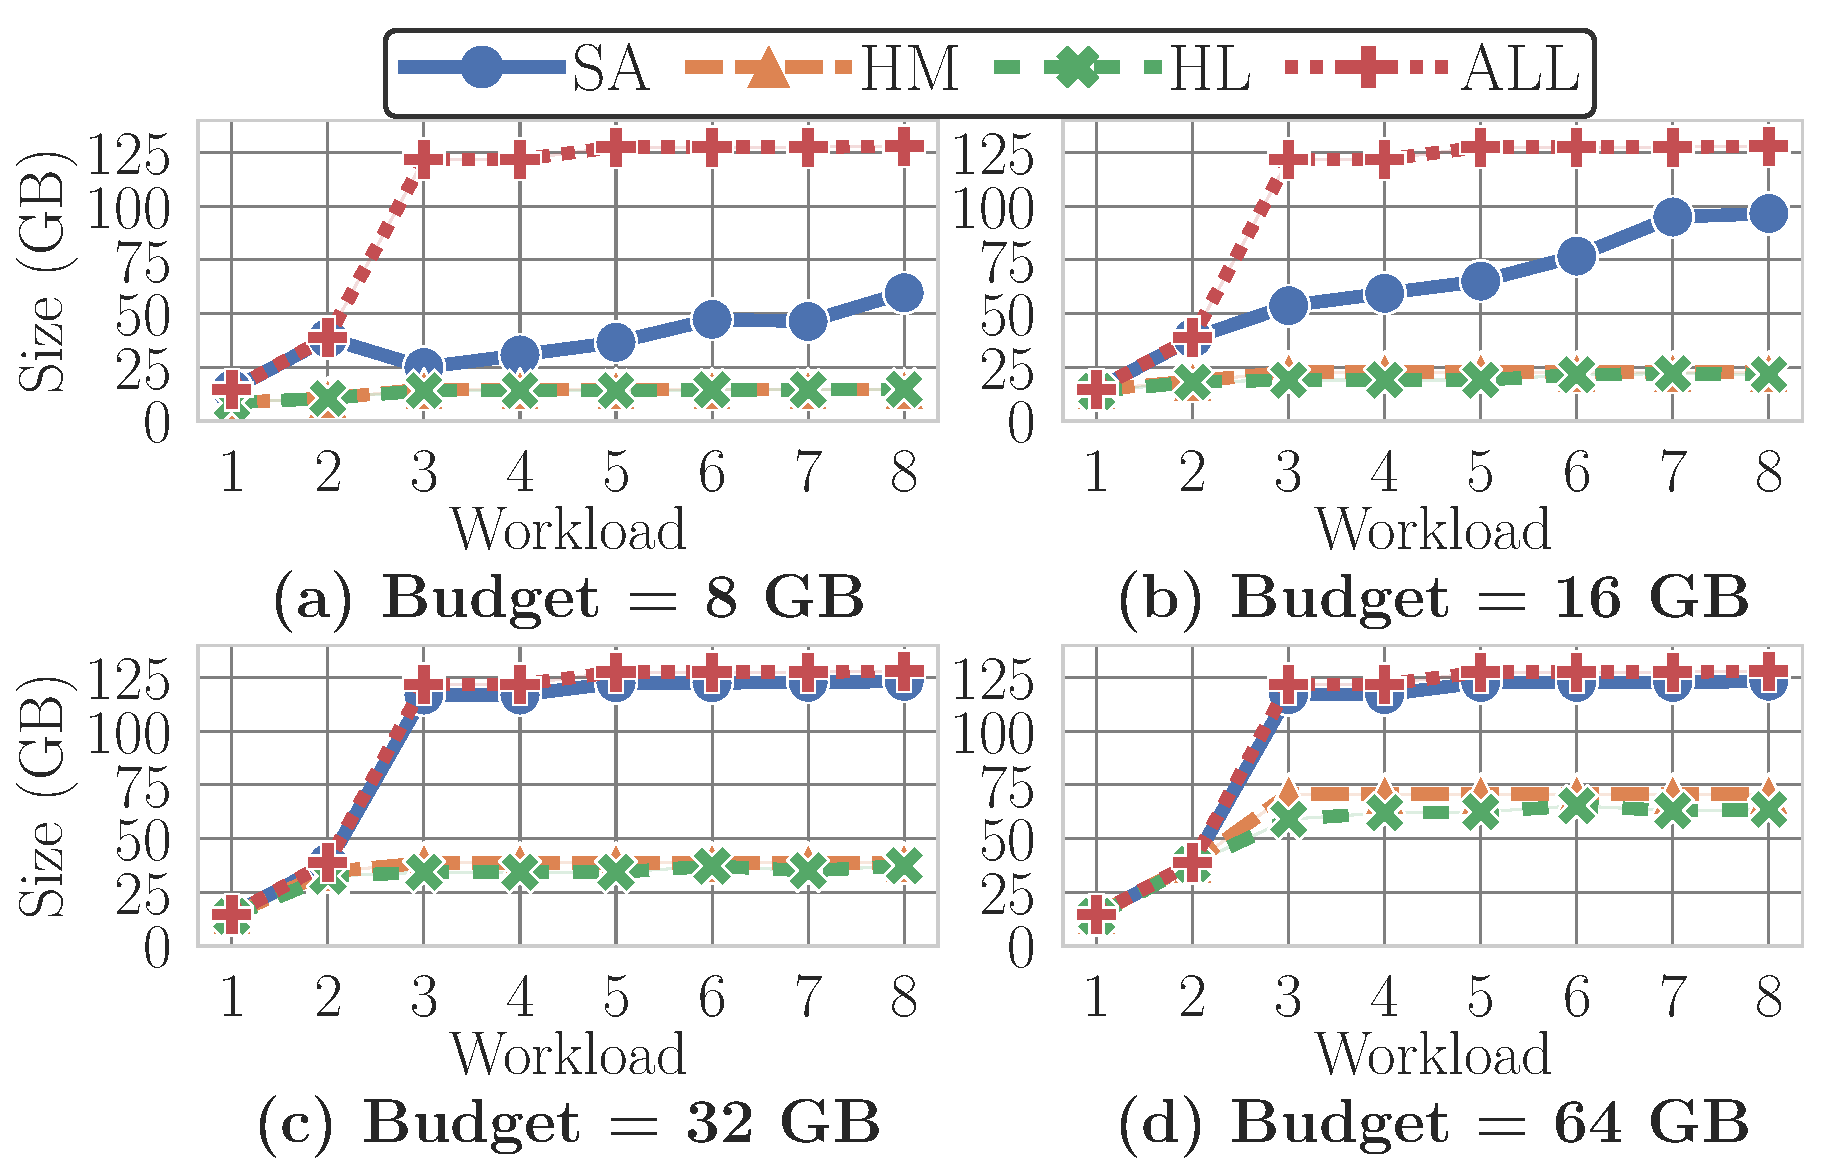
\includegraphics[width=1.0\columnwidth]{images/experiment-results/kaggle_home_credit/materialization/mat_sizes}
\caption{Real size of the materialized artifact}
\label{exp-sa-vs-simple-size}
\vspace{-4mm}
\end{figure}
\textbf{Effect of Materialization on Storage.}
In a real collaborative environment, deciding on a reasonable materialization budget requires knowledge of the expected size of the artifacts, the number of users, and the rate of incoming workloads.
In this experiment, we show that even with a small budget, our materialization algorithms, particularly our storage-aware algorithm, store a large portion of the artifacts that reappear in future workloads.
We hypothesize that there is considerable overlap between columns of different datasets in ML workloads.
Therefore, the actual total size of the artifacts that our storage-aware algorithm materializes is larger than the specified budget.

We run the Kaggle workloads under different materialization budgets and strategies.
Figures \ref{exp-sa-vs-simple-size}(a)-(d) show the real size of the stored artifacts for the heuristics-based (HM), storage-aware (SA), and Helix (HL) algorithms.
To show the total size of the materialized artifacts, we also implement a strategy that materializes every artifact in EG (represented by ALL in the figure).
In HM, the maximum real size is always equal to the budget.
This is similar for HL since it does not perform any compression or deduplication of the columns.
However, in SA, the real size of the stored artifacts reaches up to 8 times the budget.
With a materialization budget of 8 GB and 16 GB, SA materializes nearly 50\% and 80\% of all the artifacts.
For budgets larger than 16 GB, SA materializes nearly all of the artifacts.
This indicates that there is considerable overlap between the artifacts of ML workloads.
By deduplicating the artifacts, SA can materialize more artifacts.

Note that when a high-utility artifact has no overlap with other artifacts, SA still prioritizes it over other artifacts.
As a result, it is likely that when materializing an artifact that has no overlap with other artifacts, the total size of the materialized data decreases.
Figure \ref{exp-sa-vs-simple-size}(a) shows such an example.
After executing Workload 2, SA materializes several artifacts that overlap with each other.
However, in Workload 3, SA materializes a new artifact with a high utility, which represents a large dataset with many features (i.e., 1133 columns and around 3 GB).
Since the new artifact is large, SA removes many of the existing artifacts.
As a result, the total size of the materialized artifacts decreases after Workload 3.

\begin{figure}[t]
\centering
\includegraphics[width=1.0\columnwidth]{images/experiment-results/kaggle_home_credit/materialization/run-time-budget-speedup}
\caption{Total run-time and speedup (vs baseline)}
\label{run-time-vs-mat}
\vspace{-4mm}
\end{figure}
\textbf{Effect of Materialization on Run-time.}
Figure \ref{run-time-vs-mat}(a) shows the total run-time of different materialization algorithms and budgets.
ALL represents the scenario where all the artifacts are materialized.
Even with a materialization budget of 8 GB, SA has comparable performance to ALL (i.e., a difference of 100 seconds in run-time).
When the budget is larger than 8 GB, SA performs similarly to ALL.
For small materialization budgets ($\leq 16$ GB), HM performs 50\% worse than SA.
However, HM performs slightly better for larger materialization budgets.
The difference between HM and SA is because many of the artifacts are large, e.g., in Workload 3, some artifacts are more than 3 GB.
Most of these artifacts contain overlapping columns and SA compresses them.
However, HM is unable to exploit this similarity and chooses not to materialize any of the large artifacts.
Recomputing these artifacts is costly, which results in a larger run-time for HM.

HL does not prioritize the artifacts based on their cost or potential.
Thus, HL quickly exhausts the budget by materializing initial artifacts.
The impact of such behavior is more visible for smaller budgets ($\leq 16 GB$), where HL performs 20\% and 90\% worse than HM and SA, respectively.
For larger budgets, HL has similar performance to HM, since a larger fraction of all the artifacts is materialized.

In Figure \ref{run-time-vs-mat}(b), we plot the cumulative speedup (vs the KG baseline) of different materialization algorithms and budgets.
We plot the speedup of SA and HL with budgets of 8 GB and 16 GB (SA-8, SA-16, HL-8, and HL-16 in the figure) as the rest of the algorithms and budgets show similar behavior.
ALL achieves a speedup of 2 after executing all the workloads.
SA has a comparable speedup with ALL reaching speedups of 1.77 and 1.97 with budgets of 8 GB and 16 GB, respectively.
Since HL only materializes the initial artifacts, it only provides a small speedup over the KG baseline.
After executing all the workloads, HL reaches speedups of 1.11 and 1.18 with budgets of 8 GB and 16 GB.
For larger budgets (i.e., 32 GB and 64 GB), HL reaches a maximum speedup of 1.31.
Whereas, SA has a speedup of 2.0, similar to ALL.

\textbf{Effect of Model Quality on Materialization.}
In many collaborative ML use cases, users tend to utilize existing high-quality models.
In our materialization algorithm, we consider model quality when materializing an artifact.
In this experiment, we show the impact of materializing high-quality models on run-time and show that our materialization algorithm quickly detects high-quality models.

We design a model-benchmarking scenario, where users compare the score of their models with the score of the best performing model in the collaborative environment.
Such a scenario is common in collaborative environments, where users constantly attempt to improve the best current model.
We use the OpenML workloads for the model-benchmarking scenario.
The implementation of the scenario is as follows.
First, we execute the OpenML workloads one by one and keep track of the workload with the best performing model, which we refer to as the \textit{gold standard workload}.
Then, we compare every new workload with the gold standard.

Figure \ref{exp-model-materialization}(a) shows the cumulative run-time of the model-benchmarking scenario using our collaborative optimizer (CO) with default configuration (i.e., storage-aware materializer with budget 100 MB and $\alpha=0.5$) against the OpenML baseline (OML).
For every new workload, OML has to re-run the gold standard workload.
When CO encounters a gold standard workload, the materialization algorithm assigns a higher potential value to the artifacts of the workload.
As a result, such artifacts have higher materialization likelihood.
In the subsequent workloads, CO reuses the materialized artifacts of the gold standard from EG instead of re-running them, resulting in 5 times improvement in the run-time over OML.
Re-executing the gold standard workload results in an overhead of 2000 seconds, which contributes to the large run-time of OML.
In comparison, reusing the artifacts of the gold standard has an overhead of 65 seconds for CO.

We also investigate the impact of $\alpha$, which controls the importance of model quality in our materialization, on the run-time of the model-benchmarking scenario.
If $\alpha$ is close to 1, the materializer aggressively stores high-quality models.
If $\alpha$ is close to 0, the materializer prioritizes the recreation time and size over quality.
The materialization budget for the OpenML workloads is 100 MB.
However, the models in OpenML are typically small (less than 100 KB).
Therefore, regardless of the $\alpha$ value, the materializer stores the majority of the artifacts, which makes it difficult to accurately study the effect of the $\alpha$ value.
Therefore, in this experiment, we set the budget to one artifact (i.e., the materializer is only allowed to store one artifact).
An ideal materializer always selects the gold standard model.
This highlights the impact of $\alpha$ on materialization more clear.

We run the model-benchmarking scenario and vary the value of $\alpha$ from 0 to 1.
When $\alpha$ is 1, the materializer always materializes the gold standard model, as it only considers model quality.
Therefore, $\alpha=1$ incurs the smallest cumulative run-time in the model-benchmarking scenario.

In Figure \ref{exp-model-materialization}(b), we report the difference in cumulative run-time between $\alpha=1$ and other values of $\alpha$ (i.e., y-axis corresponds to the delta in cumulative run-time when compared to $\alpha=1$).
In the scenario, we repeatedly execute the gold standard; thus, the faster we materialize the gold standard model, the smaller the cumulative run-time would become.
Once we materialize the gold standard model, the delta in cumulative run-time reaches a plateau.
This is because the overhead of reusing the gold standard is negligible; thus, cumulative run-time becomes similar to when $\alpha=1$.
In workload 14, we encounter a gold standard that remains the best model until nearly the end of the experiment.
Smaller $\alpha$ values ($\alpha \leq 0.25$) materialize this model after more than 100 executions.
As a result, their delta in run-time reaches a plateau later than large $\alpha$ values ($\alpha\geq 0.5$).
The long delay in the materialization of the gold standard contributes to the higher cumulative run-time for smaller values of $\alpha$.

The default value of $\alpha$ in our system is 0.5. 
This value provides a good balance between workloads that have the goal of training high-quality models (e.g., the model-benchmarking scenario) and workloads that are more exploratory in nature.
When we have prior knowledge of the nature of the workloads, then we can set $\alpha$ accordingly.
We recommend $\alpha>0.5$ for workloads with the goal of training high-quality models and $\alpha<0.5$ for workloads with exploratory data analysis.
\begin{figure}[t]
\centering
\includegraphics[width=\columnwidth]{images/experiment-results/openml/model_materialization/model-materialization}
\caption{Effect of quality-based materialization}
\label{exp-model-materialization}
\end{figure}

\subsection{Reuse}
In this experiment, we compare our linear time reuse algorithm (LN) with Helix (HL) and two other baselines (ALL\_M and ALL\_C).
ALL\_M reuses every materialized artifact.
ALL\_C recomputes every artifact (i.e., no reuse).

Figures \ref{reuse-experiment}(a) and (b) show the run-time of the Kaggle workloads with different materialization algorithms.
ALL\_C, independent of the materialization algorithm, finishes the execution of the workloads in around 2000 seconds.
For the heuristics-based materialization, all four reuse algorithms have similar performance until Workload 6.
This is because Workload 3 has large artifacts and the heuristics-based materialization exhausts its budget by materializing them.
Furthermore, Workloads 4, 5, and 6 are modified versions of Workloads 1 and 2 (Table \ref{kaggle-workload}).
As a result, there are not many reuse opportunities until Workload 7, which is a modified version of Workload 3.
\begin{figure}[t]
\centering
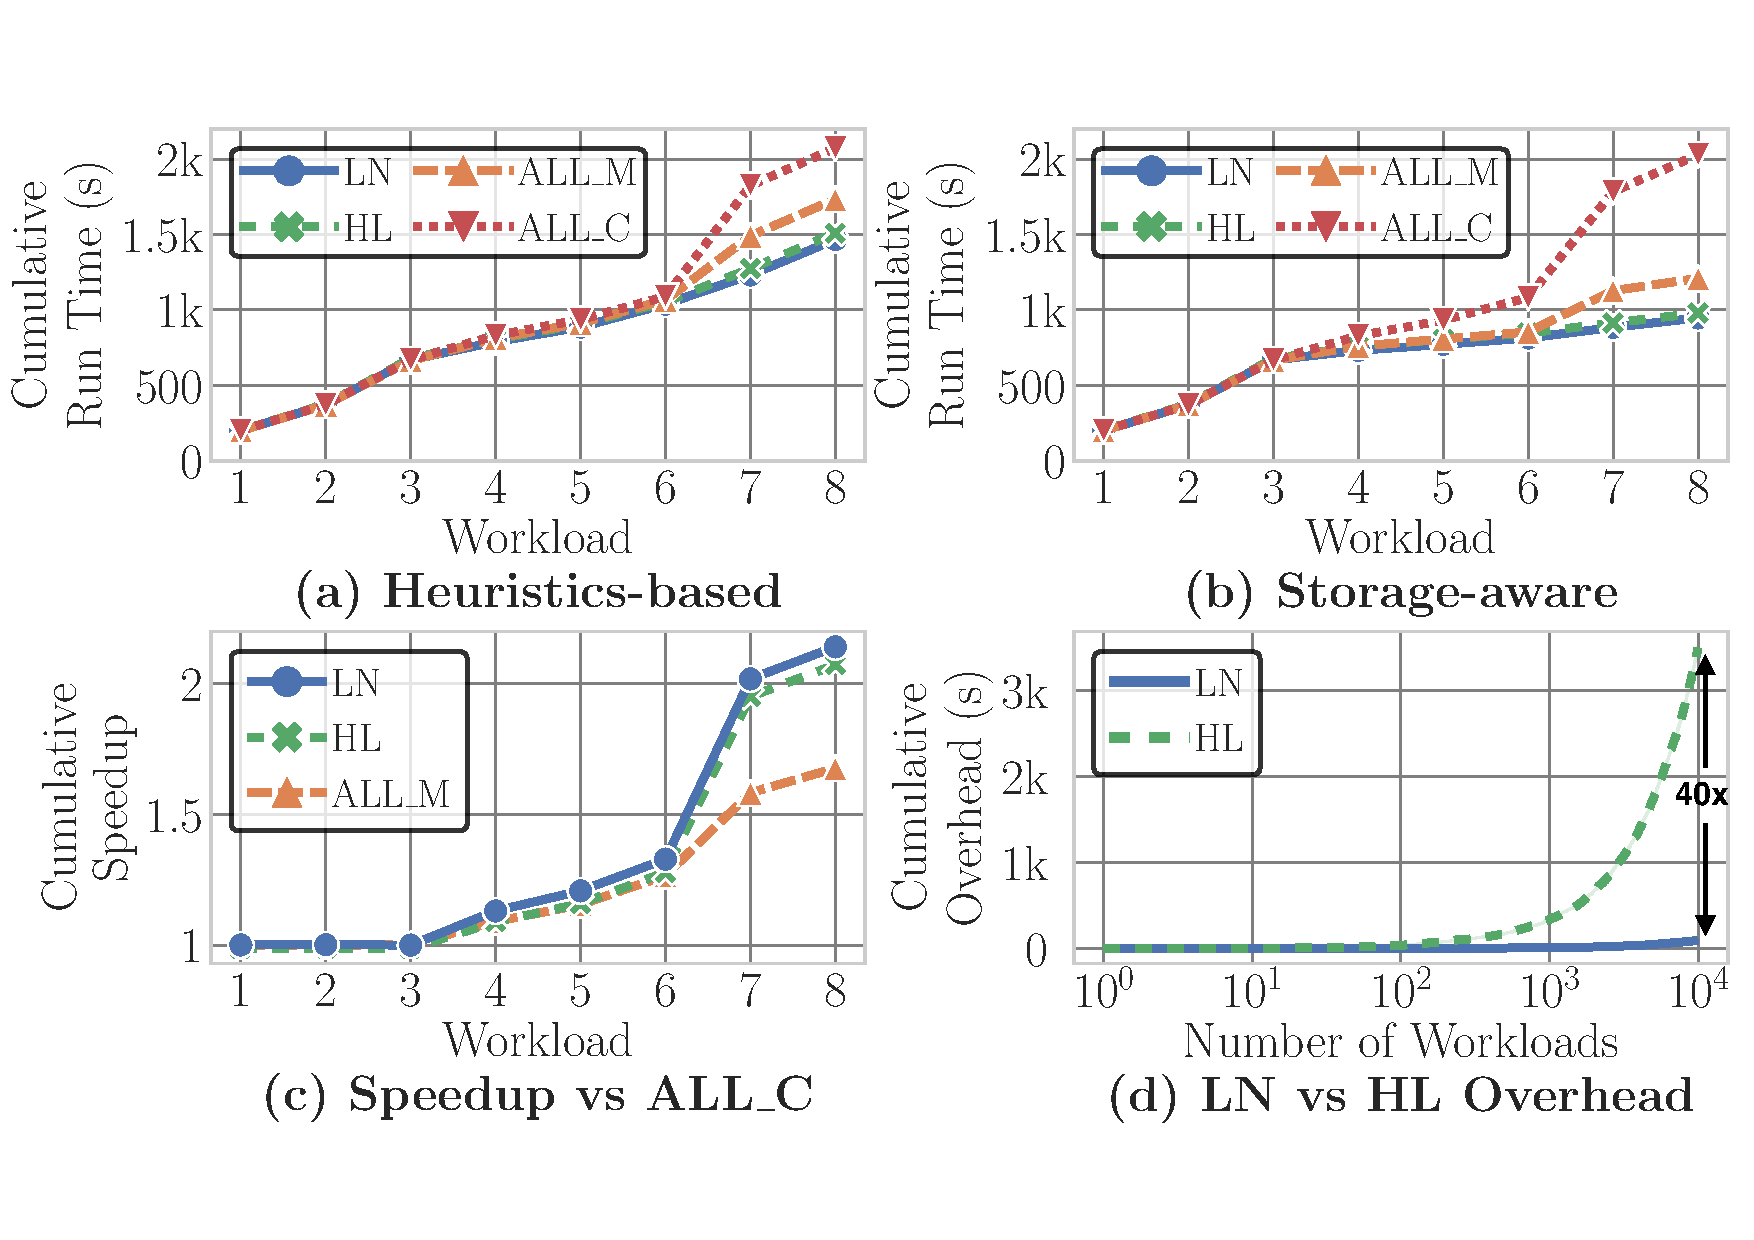
\includegraphics[width=1.0\columnwidth]{images/experiment-results/kaggle_home_credit/reuse/reuse-times-perworkload-speedups-annotated}
\caption{Run-time and overhead of reuse methods}
\label{reuse-experiment}
\vspace{-4mm}
\end{figure}

The storage-aware materialization (Figure \ref{reuse-experiment}(b)) has better budget utilization and materializes some of the artifacts of the Workloads 1 and 2.
ALL\_M, LN, and HL reuse these artifacts in Workloads 4, 5, and 6; thus, improving the run-time from Workload 4.
To better show the impact of the reuse algorithms, we plot the cumulative speedup of LN, HL, and ALL\_M over ALL\_C for the storage-aware materialization in Figure \ref{reuse-experiment}(c).
Since the first three workloads do not share many similar artifacts, the speedup is 1.
However, after the third workload, all the reuse algorithms have speedups of larger than 1.
After executing all workloads, LN and HL reach a speedup of around 2.1 with LN slightly outperforming HL.

For both materialization strategies, ALL\_M has a similar performance to LN and HL until Workload 6.
Many of the artifacts of Workload 7 incur larger load costs than compute costs.
As a result, LN and HL recompute these artifacts and result in a smaller cumulative run-time than ALL\_M, i.e., around 200-300 seconds.
In this experiment, since EG is inside the memory of the machine, load times are generally low.
LN and HL outperform ALL\_M with a larger margin in scenarios where EG is on disk.

\textbf{Reuse Overhead.} 
The polynomial-time reuse algorithm of Helix generates the same plan as our linear-time reuse.
For the Kaggle workloads, since the number and the size of workloads are relatively small, we only observe a small difference of 5 seconds in the reuse overhead. 

To show the impact of our linear-time reuse algorithm, we perform an experiment with 10,000 synthetic workloads.
We design the synthetic workloads to have similar characteristics to the real workloads in Table \ref{kaggle-workload}.
We consider the following 5 attributes of the real workload DAGs: (1) indegree distribution (i.e., join and concat operators), (2) outdegree distribution, (3) ratio of the materialized nodes, (4) distribution of the compute costs, and (5) distribution of the load costs.
A node with outdegree more than 1 represents a scenario were the node is input to different operations (e.g., training different ML models on one dataset node).
To generate the workloads, we first randomly select the number of nodes inside the workload DAG from the [500, 2000] interval, which represents many of the Kaggle workloads.
Then, for every node, we sample its attributes from the distributions of attributes of the real workloads.

Figure \ref{reuse-experiment}(d) shows the cumulative overhead of LN and HL on 10,000 generated workloads.
The overhead of LN increases linearly and after the 10,000s workloads, LN incurs a total overhead of 80 seconds.
In comparison, HL has an overhead of 3500 seconds, 40 times more than LN.
In a real collaborative environment, where hundreds of users are executing workloads, a large reuse overhead leads to slower response time and may cause a bottleneck during the optimization.
\begin{figure}[t]
\begin{subfigure}[b]{0.5\linewidth}
\centering
 \resizebox{\columnwidth}{!}{%
%% Creator: Matplotlib, PGF backend
%%
%% To include the figure in your LaTeX document, write
%%   \input{<filename>.pgf}
%%
%% Make sure the required packages are loaded in your preamble
%%   \usepackage{pgf}
%%
%% Figures using additional raster images can only be included by \input if
%% they are in the same directory as the main LaTeX file. For loading figures
%% from other directories you can use the `import` package
%%   \usepackage{import}
%% and then include the figures with
%%   \import{<path to file>}{<filename>.pgf}
%%
%% Matplotlib used the following preamble
%%   \usepackage{fontspec}
%%   \setmonofont{Andale Mono}
%%
\begingroup%
\makeatletter%
\begin{pgfpicture}%
\pgfpathrectangle{\pgfpointorigin}{\pgfqpoint{7.571861in}{4.830486in}}%
\pgfusepath{use as bounding box, clip}%
\begin{pgfscope}%
\pgfsetbuttcap%
\pgfsetmiterjoin%
\definecolor{currentfill}{rgb}{1.000000,1.000000,1.000000}%
\pgfsetfillcolor{currentfill}%
\pgfsetlinewidth{0.000000pt}%
\definecolor{currentstroke}{rgb}{1.000000,1.000000,1.000000}%
\pgfsetstrokecolor{currentstroke}%
\pgfsetdash{}{0pt}%
\pgfpathmoveto{\pgfqpoint{0.000000in}{0.000000in}}%
\pgfpathlineto{\pgfqpoint{7.571861in}{0.000000in}}%
\pgfpathlineto{\pgfqpoint{7.571861in}{4.830486in}}%
\pgfpathlineto{\pgfqpoint{0.000000in}{4.830486in}}%
\pgfpathclose%
\pgfusepath{fill}%
\end{pgfscope}%
\begin{pgfscope}%
\pgfsetbuttcap%
\pgfsetmiterjoin%
\definecolor{currentfill}{rgb}{1.000000,1.000000,1.000000}%
\pgfsetfillcolor{currentfill}%
\pgfsetlinewidth{0.000000pt}%
\definecolor{currentstroke}{rgb}{0.000000,0.000000,0.000000}%
\pgfsetstrokecolor{currentstroke}%
\pgfsetstrokeopacity{0.000000}%
\pgfsetdash{}{0pt}%
\pgfpathmoveto{\pgfqpoint{1.309444in}{1.062361in}}%
\pgfpathlineto{\pgfqpoint{6.734444in}{1.062361in}}%
\pgfpathlineto{\pgfqpoint{6.734444in}{4.082361in}}%
\pgfpathlineto{\pgfqpoint{1.309444in}{4.082361in}}%
\pgfpathclose%
\pgfusepath{fill}%
\end{pgfscope}%
\begin{pgfscope}%
\pgfpathrectangle{\pgfqpoint{1.309444in}{1.062361in}}{\pgfqpoint{5.425000in}{3.020000in}} %
\pgfusepath{clip}%
\pgfsetroundcap%
\pgfsetroundjoin%
\pgfsetlinewidth{0.803000pt}%
\definecolor{currentstroke}{rgb}{0.800000,0.800000,0.800000}%
\pgfsetstrokecolor{currentstroke}%
\pgfsetdash{}{0pt}%
\pgfpathmoveto{\pgfqpoint{1.553568in}{1.062361in}}%
\pgfpathlineto{\pgfqpoint{1.553568in}{4.082361in}}%
\pgfusepath{stroke}%
\end{pgfscope}%
\begin{pgfscope}%
\definecolor{textcolor}{rgb}{0.150000,0.150000,0.150000}%
\pgfsetstrokecolor{textcolor}%
\pgfsetfillcolor{textcolor}%
\pgftext[x=1.553568in,y=0.898472in,,top]{\color{textcolor}\rmfamily\fontsize{30.000000}{36.000000}\selectfont 0}%
\end{pgfscope}%
\begin{pgfscope}%
\pgfpathrectangle{\pgfqpoint{1.309444in}{1.062361in}}{\pgfqpoint{5.425000in}{3.020000in}} %
\pgfusepath{clip}%
\pgfsetroundcap%
\pgfsetroundjoin%
\pgfsetlinewidth{0.803000pt}%
\definecolor{currentstroke}{rgb}{0.800000,0.800000,0.800000}%
\pgfsetstrokecolor{currentstroke}%
\pgfsetdash{}{0pt}%
\pgfpathmoveto{\pgfqpoint{4.020711in}{1.062361in}}%
\pgfpathlineto{\pgfqpoint{4.020711in}{4.082361in}}%
\pgfusepath{stroke}%
\end{pgfscope}%
\begin{pgfscope}%
\definecolor{textcolor}{rgb}{0.150000,0.150000,0.150000}%
\pgfsetstrokecolor{textcolor}%
\pgfsetfillcolor{textcolor}%
\pgftext[x=4.020711in,y=0.898472in,,top]{\color{textcolor}\rmfamily\fontsize{30.000000}{36.000000}\selectfont 1000}%
\end{pgfscope}%
\begin{pgfscope}%
\pgfpathrectangle{\pgfqpoint{1.309444in}{1.062361in}}{\pgfqpoint{5.425000in}{3.020000in}} %
\pgfusepath{clip}%
\pgfsetroundcap%
\pgfsetroundjoin%
\pgfsetlinewidth{0.803000pt}%
\definecolor{currentstroke}{rgb}{0.800000,0.800000,0.800000}%
\pgfsetstrokecolor{currentstroke}%
\pgfsetdash{}{0pt}%
\pgfpathmoveto{\pgfqpoint{6.487853in}{1.062361in}}%
\pgfpathlineto{\pgfqpoint{6.487853in}{4.082361in}}%
\pgfusepath{stroke}%
\end{pgfscope}%
\begin{pgfscope}%
\definecolor{textcolor}{rgb}{0.150000,0.150000,0.150000}%
\pgfsetstrokecolor{textcolor}%
\pgfsetfillcolor{textcolor}%
\pgftext[x=6.487853in,y=0.898472in,,top]{\color{textcolor}\rmfamily\fontsize{30.000000}{36.000000}\selectfont 2000}%
\end{pgfscope}%
\begin{pgfscope}%
\definecolor{textcolor}{rgb}{0.150000,0.150000,0.150000}%
\pgfsetstrokecolor{textcolor}%
\pgfsetfillcolor{textcolor}%
\pgftext[x=4.021944in,y=0.472500in,,top]{\color{textcolor}\rmfamily\fontsize{30.000000}{36.000000}\selectfont OpenML Workload}%
\end{pgfscope}%
\begin{pgfscope}%
\pgfpathrectangle{\pgfqpoint{1.309444in}{1.062361in}}{\pgfqpoint{5.425000in}{3.020000in}} %
\pgfusepath{clip}%
\pgfsetroundcap%
\pgfsetroundjoin%
\pgfsetlinewidth{0.803000pt}%
\definecolor{currentstroke}{rgb}{0.800000,0.800000,0.800000}%
\pgfsetstrokecolor{currentstroke}%
\pgfsetdash{}{0pt}%
\pgfpathmoveto{\pgfqpoint{1.309444in}{1.181258in}}%
\pgfpathlineto{\pgfqpoint{6.734444in}{1.181258in}}%
\pgfusepath{stroke}%
\end{pgfscope}%
\begin{pgfscope}%
\definecolor{textcolor}{rgb}{0.150000,0.150000,0.150000}%
\pgfsetstrokecolor{textcolor}%
\pgfsetfillcolor{textcolor}%
\pgftext[x=0.954305in,y=1.036675in,left,base]{\color{textcolor}\rmfamily\fontsize{30.000000}{36.000000}\selectfont 0}%
\end{pgfscope}%
\begin{pgfscope}%
\pgfpathrectangle{\pgfqpoint{1.309444in}{1.062361in}}{\pgfqpoint{5.425000in}{3.020000in}} %
\pgfusepath{clip}%
\pgfsetroundcap%
\pgfsetroundjoin%
\pgfsetlinewidth{0.803000pt}%
\definecolor{currentstroke}{rgb}{0.800000,0.800000,0.800000}%
\pgfsetstrokecolor{currentstroke}%
\pgfsetdash{}{0pt}%
\pgfpathmoveto{\pgfqpoint{1.309444in}{1.906534in}}%
\pgfpathlineto{\pgfqpoint{6.734444in}{1.906534in}}%
\pgfusepath{stroke}%
\end{pgfscope}%
\begin{pgfscope}%
\definecolor{textcolor}{rgb}{0.150000,0.150000,0.150000}%
\pgfsetstrokecolor{textcolor}%
\pgfsetfillcolor{textcolor}%
\pgftext[x=0.571805in,y=1.761950in,left,base]{\color{textcolor}\rmfamily\fontsize{30.000000}{36.000000}\selectfont 200}%
\end{pgfscope}%
\begin{pgfscope}%
\pgfpathrectangle{\pgfqpoint{1.309444in}{1.062361in}}{\pgfqpoint{5.425000in}{3.020000in}} %
\pgfusepath{clip}%
\pgfsetroundcap%
\pgfsetroundjoin%
\pgfsetlinewidth{0.803000pt}%
\definecolor{currentstroke}{rgb}{0.800000,0.800000,0.800000}%
\pgfsetstrokecolor{currentstroke}%
\pgfsetdash{}{0pt}%
\pgfpathmoveto{\pgfqpoint{1.309444in}{2.631809in}}%
\pgfpathlineto{\pgfqpoint{6.734444in}{2.631809in}}%
\pgfusepath{stroke}%
\end{pgfscope}%
\begin{pgfscope}%
\definecolor{textcolor}{rgb}{0.150000,0.150000,0.150000}%
\pgfsetstrokecolor{textcolor}%
\pgfsetfillcolor{textcolor}%
\pgftext[x=0.571805in,y=2.487226in,left,base]{\color{textcolor}\rmfamily\fontsize{30.000000}{36.000000}\selectfont 400}%
\end{pgfscope}%
\begin{pgfscope}%
\pgfpathrectangle{\pgfqpoint{1.309444in}{1.062361in}}{\pgfqpoint{5.425000in}{3.020000in}} %
\pgfusepath{clip}%
\pgfsetroundcap%
\pgfsetroundjoin%
\pgfsetlinewidth{0.803000pt}%
\definecolor{currentstroke}{rgb}{0.800000,0.800000,0.800000}%
\pgfsetstrokecolor{currentstroke}%
\pgfsetdash{}{0pt}%
\pgfpathmoveto{\pgfqpoint{1.309444in}{3.357085in}}%
\pgfpathlineto{\pgfqpoint{6.734444in}{3.357085in}}%
\pgfusepath{stroke}%
\end{pgfscope}%
\begin{pgfscope}%
\definecolor{textcolor}{rgb}{0.150000,0.150000,0.150000}%
\pgfsetstrokecolor{textcolor}%
\pgfsetfillcolor{textcolor}%
\pgftext[x=0.571805in,y=3.212502in,left,base]{\color{textcolor}\rmfamily\fontsize{30.000000}{36.000000}\selectfont 600}%
\end{pgfscope}%
\begin{pgfscope}%
\pgfpathrectangle{\pgfqpoint{1.309444in}{1.062361in}}{\pgfqpoint{5.425000in}{3.020000in}} %
\pgfusepath{clip}%
\pgfsetroundcap%
\pgfsetroundjoin%
\pgfsetlinewidth{0.803000pt}%
\definecolor{currentstroke}{rgb}{0.800000,0.800000,0.800000}%
\pgfsetstrokecolor{currentstroke}%
\pgfsetdash{}{0pt}%
\pgfpathmoveto{\pgfqpoint{1.309444in}{4.082361in}}%
\pgfpathlineto{\pgfqpoint{6.734444in}{4.082361in}}%
\pgfusepath{stroke}%
\end{pgfscope}%
\begin{pgfscope}%
\definecolor{textcolor}{rgb}{0.150000,0.150000,0.150000}%
\pgfsetstrokecolor{textcolor}%
\pgfsetfillcolor{textcolor}%
\pgftext[x=0.571805in,y=3.937778in,left,base]{\color{textcolor}\rmfamily\fontsize{30.000000}{36.000000}\selectfont 800}%
\end{pgfscope}%
\begin{pgfscope}%
\definecolor{textcolor}{rgb}{0.150000,0.150000,0.150000}%
\pgfsetstrokecolor{textcolor}%
\pgfsetfillcolor{textcolor}%
\pgftext[x=0.516250in,y=2.572361in,,bottom,rotate=90.000000]{\color{textcolor}\rmfamily\fontsize{30.000000}{36.000000}\selectfont Cumulative Run Time (s)}%
\end{pgfscope}%
\begin{pgfscope}%
\pgfpathrectangle{\pgfqpoint{1.309444in}{1.062361in}}{\pgfqpoint{5.425000in}{3.020000in}} %
\pgfusepath{clip}%
\pgfsetbuttcap%
\pgfsetroundjoin%
\pgfsetlinewidth{3.011250pt}%
\definecolor{currentstroke}{rgb}{0.298039,0.447059,0.690196}%
\pgfsetstrokecolor{currentstroke}%
\pgfsetdash{{3.000000pt}{0.000000pt}}{0.000000pt}%
\pgfpathmoveto{\pgfqpoint{1.556035in}{1.187180in}}%
\pgfpathlineto{\pgfqpoint{1.563437in}{1.202274in}}%
\pgfpathlineto{\pgfqpoint{1.565904in}{1.272505in}}%
\pgfpathlineto{\pgfqpoint{1.588108in}{1.283519in}}%
\pgfpathlineto{\pgfqpoint{1.593042in}{1.288594in}}%
\pgfpathlineto{\pgfqpoint{1.627582in}{1.305056in}}%
\pgfpathlineto{\pgfqpoint{1.630049in}{1.327246in}}%
\pgfpathlineto{\pgfqpoint{1.642385in}{1.332080in}}%
\pgfpathlineto{\pgfqpoint{1.792881in}{1.335778in}}%
\pgfpathlineto{\pgfqpoint{2.486148in}{1.352199in}}%
\pgfpathlineto{\pgfqpoint{2.496016in}{1.356715in}}%
\pgfpathlineto{\pgfqpoint{2.498484in}{1.404629in}}%
\pgfpathlineto{\pgfqpoint{2.503418in}{1.406741in}}%
\pgfpathlineto{\pgfqpoint{2.508352in}{1.407018in}}%
\pgfpathlineto{\pgfqpoint{2.515754in}{1.414490in}}%
\pgfpathlineto{\pgfqpoint{2.528089in}{1.422835in}}%
\pgfpathlineto{\pgfqpoint{2.533024in}{1.424191in}}%
\pgfpathlineto{\pgfqpoint{2.542892in}{1.434270in}}%
\pgfpathlineto{\pgfqpoint{2.545359in}{1.437180in}}%
\pgfpathlineto{\pgfqpoint{2.552761in}{1.439773in}}%
\pgfpathlineto{\pgfqpoint{2.562629in}{1.447243in}}%
\pgfpathlineto{\pgfqpoint{2.565096in}{1.447730in}}%
\pgfpathlineto{\pgfqpoint{2.570031in}{1.451040in}}%
\pgfpathlineto{\pgfqpoint{2.577432in}{1.452429in}}%
\pgfpathlineto{\pgfqpoint{2.582366in}{1.454602in}}%
\pgfpathlineto{\pgfqpoint{2.584834in}{1.455374in}}%
\pgfpathlineto{\pgfqpoint{2.589768in}{1.458940in}}%
\pgfpathlineto{\pgfqpoint{2.592235in}{1.459364in}}%
\pgfpathlineto{\pgfqpoint{2.599636in}{1.464391in}}%
\pgfpathlineto{\pgfqpoint{2.604571in}{1.466594in}}%
\pgfpathlineto{\pgfqpoint{2.607038in}{1.469716in}}%
\pgfpathlineto{\pgfqpoint{2.609505in}{1.470344in}}%
\pgfpathlineto{\pgfqpoint{2.616906in}{1.477726in}}%
\pgfpathlineto{\pgfqpoint{2.648979in}{1.491148in}}%
\pgfpathlineto{\pgfqpoint{2.653914in}{1.496726in}}%
\pgfpathlineto{\pgfqpoint{2.668716in}{1.503321in}}%
\pgfpathlineto{\pgfqpoint{2.671184in}{1.505946in}}%
\pgfpathlineto{\pgfqpoint{2.673651in}{1.506264in}}%
\pgfpathlineto{\pgfqpoint{2.681052in}{1.511074in}}%
\pgfpathlineto{\pgfqpoint{2.688454in}{1.513706in}}%
\pgfpathlineto{\pgfqpoint{2.705724in}{1.521056in}}%
\pgfpathlineto{\pgfqpoint{2.722994in}{1.523195in}}%
\pgfpathlineto{\pgfqpoint{2.727928in}{1.525129in}}%
\pgfpathlineto{\pgfqpoint{3.909689in}{1.619563in}}%
\pgfpathlineto{\pgfqpoint{3.934361in}{1.622103in}}%
\pgfpathlineto{\pgfqpoint{4.876809in}{1.696312in}}%
\pgfpathlineto{\pgfqpoint{4.879276in}{1.700379in}}%
\pgfpathlineto{\pgfqpoint{5.138326in}{1.721205in}}%
\pgfpathlineto{\pgfqpoint{5.143261in}{1.722890in}}%
\pgfpathlineto{\pgfqpoint{5.422048in}{1.746312in}}%
\pgfpathlineto{\pgfqpoint{5.431916in}{1.747580in}}%
\pgfpathlineto{\pgfqpoint{5.473858in}{1.752133in}}%
\pgfpathlineto{\pgfqpoint{5.488660in}{1.755021in}}%
\pgfpathlineto{\pgfqpoint{5.602149in}{1.765285in}}%
\pgfpathlineto{\pgfqpoint{5.607083in}{1.766929in}}%
\pgfpathlineto{\pgfqpoint{5.631755in}{1.769363in}}%
\pgfpathlineto{\pgfqpoint{5.636689in}{1.771066in}}%
\pgfpathlineto{\pgfqpoint{5.715638in}{1.778749in}}%
\pgfpathlineto{\pgfqpoint{5.725506in}{1.780021in}}%
\pgfpathlineto{\pgfqpoint{5.801988in}{1.786551in}}%
\pgfpathlineto{\pgfqpoint{5.806922in}{1.788195in}}%
\pgfpathlineto{\pgfqpoint{5.977155in}{1.802187in}}%
\pgfpathlineto{\pgfqpoint{5.982089in}{1.803798in}}%
\pgfpathlineto{\pgfqpoint{5.989490in}{1.804881in}}%
\pgfpathlineto{\pgfqpoint{5.994425in}{1.806451in}}%
\pgfpathlineto{\pgfqpoint{6.186862in}{1.823112in}}%
\pgfpathlineto{\pgfqpoint{6.189329in}{1.991122in}}%
\pgfpathlineto{\pgfqpoint{6.263343in}{1.997502in}}%
\pgfpathlineto{\pgfqpoint{6.268278in}{1.999067in}}%
\pgfpathlineto{\pgfqpoint{6.401503in}{2.010582in}}%
\pgfpathlineto{\pgfqpoint{6.411372in}{2.011853in}}%
\pgfpathlineto{\pgfqpoint{6.487853in}{2.019142in}}%
\pgfpathlineto{\pgfqpoint{6.487853in}{2.019142in}}%
\pgfusepath{stroke}%
\end{pgfscope}%
\begin{pgfscope}%
\pgfpathrectangle{\pgfqpoint{1.309444in}{1.062361in}}{\pgfqpoint{5.425000in}{3.020000in}} %
\pgfusepath{clip}%
\pgfsetbuttcap%
\pgfsetroundjoin%
\pgfsetlinewidth{3.011250pt}%
\definecolor{currentstroke}{rgb}{0.866667,0.517647,0.321569}%
\pgfsetstrokecolor{currentstroke}%
\pgfsetdash{{3.000000pt}{3.000000pt}}{0.000000pt}%
\pgfpathmoveto{\pgfqpoint{1.556035in}{1.187252in}}%
\pgfpathlineto{\pgfqpoint{1.563437in}{1.203047in}}%
\pgfpathlineto{\pgfqpoint{1.565904in}{1.254982in}}%
\pgfpathlineto{\pgfqpoint{1.585641in}{1.304136in}}%
\pgfpathlineto{\pgfqpoint{1.588108in}{1.305150in}}%
\pgfpathlineto{\pgfqpoint{1.600444in}{1.324342in}}%
\pgfpathlineto{\pgfqpoint{1.625115in}{1.403733in}}%
\pgfpathlineto{\pgfqpoint{1.627582in}{1.408924in}}%
\pgfpathlineto{\pgfqpoint{1.632516in}{1.446062in}}%
\pgfpathlineto{\pgfqpoint{1.639918in}{1.465981in}}%
\pgfpathlineto{\pgfqpoint{1.691728in}{1.467428in}}%
\pgfpathlineto{\pgfqpoint{2.486148in}{1.488575in}}%
\pgfpathlineto{\pgfqpoint{2.496016in}{1.492955in}}%
\pgfpathlineto{\pgfqpoint{2.498484in}{1.540866in}}%
\pgfpathlineto{\pgfqpoint{2.503418in}{1.543037in}}%
\pgfpathlineto{\pgfqpoint{2.508352in}{1.543283in}}%
\pgfpathlineto{\pgfqpoint{2.515754in}{1.550686in}}%
\pgfpathlineto{\pgfqpoint{2.528089in}{1.558944in}}%
\pgfpathlineto{\pgfqpoint{2.533024in}{1.560248in}}%
\pgfpathlineto{\pgfqpoint{2.540425in}{1.568285in}}%
\pgfpathlineto{\pgfqpoint{2.547826in}{1.574106in}}%
\pgfpathlineto{\pgfqpoint{2.555228in}{1.578608in}}%
\pgfpathlineto{\pgfqpoint{2.570031in}{1.587410in}}%
\pgfpathlineto{\pgfqpoint{2.577432in}{1.588849in}}%
\pgfpathlineto{\pgfqpoint{2.582366in}{1.591024in}}%
\pgfpathlineto{\pgfqpoint{2.584834in}{1.591806in}}%
\pgfpathlineto{\pgfqpoint{2.589768in}{1.595364in}}%
\pgfpathlineto{\pgfqpoint{2.592235in}{1.595808in}}%
\pgfpathlineto{\pgfqpoint{2.599636in}{1.600903in}}%
\pgfpathlineto{\pgfqpoint{2.604571in}{1.603112in}}%
\pgfpathlineto{\pgfqpoint{2.611972in}{1.609887in}}%
\pgfpathlineto{\pgfqpoint{2.616906in}{1.614085in}}%
\pgfpathlineto{\pgfqpoint{2.648979in}{1.628021in}}%
\pgfpathlineto{\pgfqpoint{2.653914in}{1.633518in}}%
\pgfpathlineto{\pgfqpoint{2.668716in}{1.640105in}}%
\pgfpathlineto{\pgfqpoint{2.671184in}{1.642685in}}%
\pgfpathlineto{\pgfqpoint{2.673651in}{1.643017in}}%
\pgfpathlineto{\pgfqpoint{2.681052in}{1.647774in}}%
\pgfpathlineto{\pgfqpoint{2.688454in}{1.650422in}}%
\pgfpathlineto{\pgfqpoint{2.708191in}{1.659321in}}%
\pgfpathlineto{\pgfqpoint{2.722994in}{1.666630in}}%
\pgfpathlineto{\pgfqpoint{2.730395in}{1.670362in}}%
\pgfpathlineto{\pgfqpoint{2.824146in}{1.719070in}}%
\pgfpathlineto{\pgfqpoint{2.838949in}{1.725908in}}%
\pgfpathlineto{\pgfqpoint{2.848818in}{1.730465in}}%
\pgfpathlineto{\pgfqpoint{2.866088in}{1.737390in}}%
\pgfpathlineto{\pgfqpoint{2.890759in}{1.752548in}}%
\pgfpathlineto{\pgfqpoint{2.898161in}{1.756107in}}%
\pgfpathlineto{\pgfqpoint{2.905562in}{1.761712in}}%
\pgfpathlineto{\pgfqpoint{2.917898in}{1.769583in}}%
\pgfpathlineto{\pgfqpoint{2.937635in}{1.779013in}}%
\pgfpathlineto{\pgfqpoint{2.994379in}{1.806598in}}%
\pgfpathlineto{\pgfqpoint{3.004248in}{1.811404in}}%
\pgfpathlineto{\pgfqpoint{3.031386in}{1.824061in}}%
\pgfpathlineto{\pgfqpoint{3.041255in}{1.828766in}}%
\pgfpathlineto{\pgfqpoint{3.056058in}{1.835038in}}%
\pgfpathlineto{\pgfqpoint{3.088131in}{1.853037in}}%
\pgfpathlineto{\pgfqpoint{3.105401in}{1.862840in}}%
\pgfpathlineto{\pgfqpoint{3.132539in}{1.878198in}}%
\pgfpathlineto{\pgfqpoint{3.273166in}{1.947419in}}%
\pgfpathlineto{\pgfqpoint{3.283035in}{1.952423in}}%
\pgfpathlineto{\pgfqpoint{3.315108in}{1.967118in}}%
\pgfpathlineto{\pgfqpoint{3.332378in}{1.975020in}}%
\pgfpathlineto{\pgfqpoint{3.357049in}{1.987070in}}%
\pgfpathlineto{\pgfqpoint{3.369385in}{1.993508in}}%
\pgfpathlineto{\pgfqpoint{3.394056in}{2.005372in}}%
\pgfpathlineto{\pgfqpoint{3.401458in}{2.008293in}}%
\pgfpathlineto{\pgfqpoint{3.408859in}{2.011533in}}%
\pgfpathlineto{\pgfqpoint{3.421195in}{2.018618in}}%
\pgfpathlineto{\pgfqpoint{3.431063in}{2.023729in}}%
\pgfpathlineto{\pgfqpoint{3.460669in}{2.037770in}}%
\pgfpathlineto{\pgfqpoint{3.480406in}{2.047481in}}%
\pgfpathlineto{\pgfqpoint{3.502611in}{2.058429in}}%
\pgfpathlineto{\pgfqpoint{3.510012in}{2.061826in}}%
\pgfpathlineto{\pgfqpoint{3.524815in}{2.068969in}}%
\pgfpathlineto{\pgfqpoint{3.576625in}{2.093507in}}%
\pgfpathlineto{\pgfqpoint{3.588961in}{2.099079in}}%
\pgfpathlineto{\pgfqpoint{3.603763in}{2.107293in}}%
\pgfpathlineto{\pgfqpoint{3.845543in}{2.226652in}}%
\pgfpathlineto{\pgfqpoint{3.852945in}{2.231328in}}%
\pgfpathlineto{\pgfqpoint{3.867748in}{2.237490in}}%
\pgfpathlineto{\pgfqpoint{3.909689in}{2.257621in}}%
\pgfpathlineto{\pgfqpoint{3.919558in}{2.262172in}}%
\pgfpathlineto{\pgfqpoint{3.924492in}{2.265221in}}%
\pgfpathlineto{\pgfqpoint{3.936828in}{2.270616in}}%
\pgfpathlineto{\pgfqpoint{3.951631in}{2.279153in}}%
\pgfpathlineto{\pgfqpoint{4.025645in}{2.315109in}}%
\pgfpathlineto{\pgfqpoint{4.033046in}{2.319416in}}%
\pgfpathlineto{\pgfqpoint{4.084856in}{2.345521in}}%
\pgfpathlineto{\pgfqpoint{4.094725in}{2.351369in}}%
\pgfpathlineto{\pgfqpoint{4.102126in}{2.355310in}}%
\pgfpathlineto{\pgfqpoint{4.134199in}{2.370481in}}%
\pgfpathlineto{\pgfqpoint{4.161338in}{2.385264in}}%
\pgfpathlineto{\pgfqpoint{4.183542in}{2.395571in}}%
\pgfpathlineto{\pgfqpoint{4.190943in}{2.399167in}}%
\pgfpathlineto{\pgfqpoint{4.200812in}{2.405682in}}%
\pgfpathlineto{\pgfqpoint{4.223016in}{2.416878in}}%
\pgfpathlineto{\pgfqpoint{4.237819in}{2.425102in}}%
\pgfpathlineto{\pgfqpoint{4.260023in}{2.435214in}}%
\pgfpathlineto{\pgfqpoint{4.272359in}{2.442557in}}%
\pgfpathlineto{\pgfqpoint{4.282228in}{2.447200in}}%
\pgfpathlineto{\pgfqpoint{4.442592in}{2.527087in}}%
\pgfpathlineto{\pgfqpoint{4.454928in}{2.534151in}}%
\pgfpathlineto{\pgfqpoint{4.479599in}{2.546174in}}%
\pgfpathlineto{\pgfqpoint{4.496869in}{2.554480in}}%
\pgfpathlineto{\pgfqpoint{4.504271in}{2.558611in}}%
\pgfpathlineto{\pgfqpoint{4.526475in}{2.570111in}}%
\pgfpathlineto{\pgfqpoint{4.536343in}{2.575213in}}%
\pgfpathlineto{\pgfqpoint{4.570883in}{2.590425in}}%
\pgfpathlineto{\pgfqpoint{4.583219in}{2.595464in}}%
\pgfpathlineto{\pgfqpoint{4.590621in}{2.599375in}}%
\pgfpathlineto{\pgfqpoint{4.610358in}{2.608213in}}%
\pgfpathlineto{\pgfqpoint{4.620226in}{2.614448in}}%
\pgfpathlineto{\pgfqpoint{4.647365in}{2.625864in}}%
\pgfpathlineto{\pgfqpoint{4.664635in}{2.636574in}}%
\pgfpathlineto{\pgfqpoint{4.676971in}{2.642227in}}%
\pgfpathlineto{\pgfqpoint{4.689306in}{2.648013in}}%
\pgfpathlineto{\pgfqpoint{4.704109in}{2.655774in}}%
\pgfpathlineto{\pgfqpoint{4.711511in}{2.660971in}}%
\pgfpathlineto{\pgfqpoint{4.723846in}{2.667273in}}%
\pgfpathlineto{\pgfqpoint{4.746051in}{2.676858in}}%
\pgfpathlineto{\pgfqpoint{4.763321in}{2.683939in}}%
\pgfpathlineto{\pgfqpoint{4.876809in}{2.735729in}}%
\pgfpathlineto{\pgfqpoint{4.879276in}{2.739810in}}%
\pgfpathlineto{\pgfqpoint{4.894079in}{2.747218in}}%
\pgfpathlineto{\pgfqpoint{4.908882in}{2.754038in}}%
\pgfpathlineto{\pgfqpoint{4.943422in}{2.769978in}}%
\pgfpathlineto{\pgfqpoint{5.197538in}{2.890815in}}%
\pgfpathlineto{\pgfqpoint{5.204939in}{2.894390in}}%
\pgfpathlineto{\pgfqpoint{5.259216in}{2.922034in}}%
\pgfpathlineto{\pgfqpoint{5.266618in}{2.926123in}}%
\pgfpathlineto{\pgfqpoint{5.276486in}{2.931011in}}%
\pgfpathlineto{\pgfqpoint{5.293756in}{2.938773in}}%
\pgfpathlineto{\pgfqpoint{5.320895in}{2.950719in}}%
\pgfpathlineto{\pgfqpoint{5.340632in}{2.958775in}}%
\pgfpathlineto{\pgfqpoint{5.360369in}{2.968029in}}%
\pgfpathlineto{\pgfqpoint{5.385040in}{2.977893in}}%
\pgfpathlineto{\pgfqpoint{5.389975in}{2.981227in}}%
\pgfpathlineto{\pgfqpoint{5.446719in}{3.007527in}}%
\pgfpathlineto{\pgfqpoint{5.463989in}{3.016896in}}%
\pgfpathlineto{\pgfqpoint{5.496062in}{3.032832in}}%
\pgfpathlineto{\pgfqpoint{5.513332in}{3.039772in}}%
\pgfpathlineto{\pgfqpoint{5.528135in}{3.047172in}}%
\pgfpathlineto{\pgfqpoint{5.602149in}{3.082287in}}%
\pgfpathlineto{\pgfqpoint{5.614485in}{3.087907in}}%
\pgfpathlineto{\pgfqpoint{5.634222in}{3.098613in}}%
\pgfpathlineto{\pgfqpoint{5.644090in}{3.103672in}}%
\pgfpathlineto{\pgfqpoint{6.028965in}{3.287003in}}%
\pgfpathlineto{\pgfqpoint{6.041300in}{3.292787in}}%
\pgfpathlineto{\pgfqpoint{6.048702in}{3.297485in}}%
\pgfpathlineto{\pgfqpoint{6.056103in}{3.301275in}}%
\pgfpathlineto{\pgfqpoint{6.078308in}{3.313080in}}%
\pgfpathlineto{\pgfqpoint{6.090643in}{3.319170in}}%
\pgfpathlineto{\pgfqpoint{6.110380in}{3.329289in}}%
\pgfpathlineto{\pgfqpoint{6.127650in}{3.337963in}}%
\pgfpathlineto{\pgfqpoint{6.139986in}{3.346065in}}%
\pgfpathlineto{\pgfqpoint{6.144920in}{3.348854in}}%
\pgfpathlineto{\pgfqpoint{6.159723in}{3.356773in}}%
\pgfpathlineto{\pgfqpoint{6.181928in}{3.365937in}}%
\pgfpathlineto{\pgfqpoint{6.186862in}{3.368996in}}%
\pgfpathlineto{\pgfqpoint{6.189329in}{3.536643in}}%
\pgfpathlineto{\pgfqpoint{6.199198in}{3.542776in}}%
\pgfpathlineto{\pgfqpoint{6.280613in}{3.581784in}}%
\pgfpathlineto{\pgfqpoint{6.305285in}{3.593070in}}%
\pgfpathlineto{\pgfqpoint{6.312686in}{3.596384in}}%
\pgfpathlineto{\pgfqpoint{6.322555in}{3.602004in}}%
\pgfpathlineto{\pgfqpoint{6.337358in}{3.609792in}}%
\pgfpathlineto{\pgfqpoint{6.352160in}{3.616644in}}%
\pgfpathlineto{\pgfqpoint{6.366963in}{3.622599in}}%
\pgfpathlineto{\pgfqpoint{6.399036in}{3.636715in}}%
\pgfpathlineto{\pgfqpoint{6.403970in}{3.639640in}}%
\pgfpathlineto{\pgfqpoint{6.445912in}{3.660633in}}%
\pgfpathlineto{\pgfqpoint{6.453313in}{3.665986in}}%
\pgfpathlineto{\pgfqpoint{6.465649in}{3.671805in}}%
\pgfpathlineto{\pgfqpoint{6.473050in}{3.676694in}}%
\pgfpathlineto{\pgfqpoint{6.487853in}{3.683557in}}%
\pgfpathlineto{\pgfqpoint{6.487853in}{3.683557in}}%
\pgfusepath{stroke}%
\end{pgfscope}%
\begin{pgfscope}%
\pgfpathrectangle{\pgfqpoint{1.309444in}{1.062361in}}{\pgfqpoint{5.425000in}{3.020000in}} %
\pgfusepath{clip}%
\pgfsetbuttcap%
\pgfsetroundjoin%
\pgfsetlinewidth{3.011250pt}%
\definecolor{currentstroke}{rgb}{0.333333,0.658824,0.407843}%
\pgfsetstrokecolor{currentstroke}%
\pgfsetdash{{6.000000pt}{3.000000pt}}{0.000000pt}%
\pgfpathmoveto{\pgfqpoint{1.556035in}{1.187189in}}%
\pgfpathlineto{\pgfqpoint{1.563437in}{1.202950in}}%
\pgfpathlineto{\pgfqpoint{1.565904in}{1.274217in}}%
\pgfpathlineto{\pgfqpoint{1.585641in}{1.323251in}}%
\pgfpathlineto{\pgfqpoint{1.588108in}{1.324244in}}%
\pgfpathlineto{\pgfqpoint{1.595509in}{1.336018in}}%
\pgfpathlineto{\pgfqpoint{1.597977in}{1.337163in}}%
\pgfpathlineto{\pgfqpoint{1.602911in}{1.351206in}}%
\pgfpathlineto{\pgfqpoint{1.612779in}{1.381528in}}%
\pgfpathlineto{\pgfqpoint{1.615246in}{1.381586in}}%
\pgfpathlineto{\pgfqpoint{1.620181in}{1.393870in}}%
\pgfpathlineto{\pgfqpoint{1.625115in}{1.410025in}}%
\pgfpathlineto{\pgfqpoint{1.627582in}{1.415242in}}%
\pgfpathlineto{\pgfqpoint{1.632516in}{1.450961in}}%
\pgfpathlineto{\pgfqpoint{1.639918in}{1.470378in}}%
\pgfpathlineto{\pgfqpoint{2.049464in}{1.480230in}}%
\pgfpathlineto{\pgfqpoint{2.486148in}{1.490588in}}%
\pgfpathlineto{\pgfqpoint{2.496016in}{1.495156in}}%
\pgfpathlineto{\pgfqpoint{2.498484in}{1.542995in}}%
\pgfpathlineto{\pgfqpoint{2.503418in}{1.545181in}}%
\pgfpathlineto{\pgfqpoint{2.508352in}{1.545455in}}%
\pgfpathlineto{\pgfqpoint{2.515754in}{1.552713in}}%
\pgfpathlineto{\pgfqpoint{2.528089in}{1.560789in}}%
\pgfpathlineto{\pgfqpoint{2.533024in}{1.562117in}}%
\pgfpathlineto{\pgfqpoint{2.542892in}{1.571955in}}%
\pgfpathlineto{\pgfqpoint{2.545359in}{1.574669in}}%
\pgfpathlineto{\pgfqpoint{2.552761in}{1.577166in}}%
\pgfpathlineto{\pgfqpoint{2.562629in}{1.584449in}}%
\pgfpathlineto{\pgfqpoint{2.565096in}{1.584960in}}%
\pgfpathlineto{\pgfqpoint{2.570031in}{1.588173in}}%
\pgfpathlineto{\pgfqpoint{2.577432in}{1.589535in}}%
\pgfpathlineto{\pgfqpoint{2.582366in}{1.591654in}}%
\pgfpathlineto{\pgfqpoint{2.584834in}{1.592411in}}%
\pgfpathlineto{\pgfqpoint{2.589768in}{1.595939in}}%
\pgfpathlineto{\pgfqpoint{2.594702in}{1.598336in}}%
\pgfpathlineto{\pgfqpoint{2.597169in}{1.598897in}}%
\pgfpathlineto{\pgfqpoint{2.602104in}{1.601907in}}%
\pgfpathlineto{\pgfqpoint{2.609505in}{1.607082in}}%
\pgfpathlineto{\pgfqpoint{2.616906in}{1.614242in}}%
\pgfpathlineto{\pgfqpoint{2.648979in}{1.627283in}}%
\pgfpathlineto{\pgfqpoint{2.653914in}{1.632703in}}%
\pgfpathlineto{\pgfqpoint{2.668716in}{1.639113in}}%
\pgfpathlineto{\pgfqpoint{2.671184in}{1.641658in}}%
\pgfpathlineto{\pgfqpoint{2.673651in}{1.641965in}}%
\pgfpathlineto{\pgfqpoint{2.681052in}{1.646618in}}%
\pgfpathlineto{\pgfqpoint{2.688454in}{1.649175in}}%
\pgfpathlineto{\pgfqpoint{2.708191in}{1.657719in}}%
\pgfpathlineto{\pgfqpoint{2.722994in}{1.664834in}}%
\pgfpathlineto{\pgfqpoint{2.730395in}{1.668470in}}%
\pgfpathlineto{\pgfqpoint{2.752599in}{1.678610in}}%
\pgfpathlineto{\pgfqpoint{2.762468in}{1.683416in}}%
\pgfpathlineto{\pgfqpoint{2.772336in}{1.689312in}}%
\pgfpathlineto{\pgfqpoint{2.801942in}{1.704306in}}%
\pgfpathlineto{\pgfqpoint{2.811811in}{1.709602in}}%
\pgfpathlineto{\pgfqpoint{2.898161in}{1.750212in}}%
\pgfpathlineto{\pgfqpoint{2.905562in}{1.755209in}}%
\pgfpathlineto{\pgfqpoint{2.954905in}{1.778907in}}%
\pgfpathlineto{\pgfqpoint{2.967241in}{1.785459in}}%
\pgfpathlineto{\pgfqpoint{2.991912in}{1.796893in}}%
\pgfpathlineto{\pgfqpoint{3.063459in}{1.830586in}}%
\pgfpathlineto{\pgfqpoint{3.073328in}{1.835665in}}%
\pgfpathlineto{\pgfqpoint{3.095532in}{1.847300in}}%
\pgfpathlineto{\pgfqpoint{3.100466in}{1.850265in}}%
\pgfpathlineto{\pgfqpoint{3.110335in}{1.855502in}}%
\pgfpathlineto{\pgfqpoint{3.130072in}{1.867024in}}%
\pgfpathlineto{\pgfqpoint{3.142408in}{1.872481in}}%
\pgfpathlineto{\pgfqpoint{3.149809in}{1.876835in}}%
\pgfpathlineto{\pgfqpoint{3.172014in}{1.887591in}}%
\pgfpathlineto{\pgfqpoint{3.238626in}{1.918275in}}%
\pgfpathlineto{\pgfqpoint{3.270699in}{1.934942in}}%
\pgfpathlineto{\pgfqpoint{3.292904in}{1.945573in}}%
\pgfpathlineto{\pgfqpoint{3.495209in}{2.041816in}}%
\pgfpathlineto{\pgfqpoint{3.507545in}{2.047496in}}%
\pgfpathlineto{\pgfqpoint{3.532216in}{2.059064in}}%
\pgfpathlineto{\pgfqpoint{3.547019in}{2.066893in}}%
\pgfpathlineto{\pgfqpoint{3.556888in}{2.071642in}}%
\pgfpathlineto{\pgfqpoint{3.574158in}{2.078901in}}%
\pgfpathlineto{\pgfqpoint{3.586493in}{2.083925in}}%
\pgfpathlineto{\pgfqpoint{4.146535in}{2.357460in}}%
\pgfpathlineto{\pgfqpoint{4.161338in}{2.365352in}}%
\pgfpathlineto{\pgfqpoint{4.183542in}{2.375629in}}%
\pgfpathlineto{\pgfqpoint{4.190943in}{2.379210in}}%
\pgfpathlineto{\pgfqpoint{4.200812in}{2.385757in}}%
\pgfpathlineto{\pgfqpoint{4.232885in}{2.401545in}}%
\pgfpathlineto{\pgfqpoint{4.240286in}{2.405621in}}%
\pgfpathlineto{\pgfqpoint{4.329103in}{2.448300in}}%
\pgfpathlineto{\pgfqpoint{4.343906in}{2.455872in}}%
\pgfpathlineto{\pgfqpoint{4.361176in}{2.465107in}}%
\pgfpathlineto{\pgfqpoint{4.385848in}{2.475886in}}%
\pgfpathlineto{\pgfqpoint{4.395716in}{2.481039in}}%
\pgfpathlineto{\pgfqpoint{4.410519in}{2.489144in}}%
\pgfpathlineto{\pgfqpoint{4.427789in}{2.497371in}}%
\pgfpathlineto{\pgfqpoint{4.447526in}{2.509371in}}%
\pgfpathlineto{\pgfqpoint{4.457395in}{2.514346in}}%
\pgfpathlineto{\pgfqpoint{4.494402in}{2.531865in}}%
\pgfpathlineto{\pgfqpoint{4.521541in}{2.546219in}}%
\pgfpathlineto{\pgfqpoint{4.558548in}{2.564518in}}%
\pgfpathlineto{\pgfqpoint{4.583219in}{2.574324in}}%
\pgfpathlineto{\pgfqpoint{4.590621in}{2.578214in}}%
\pgfpathlineto{\pgfqpoint{4.610358in}{2.587108in}}%
\pgfpathlineto{\pgfqpoint{4.620226in}{2.593333in}}%
\pgfpathlineto{\pgfqpoint{4.647365in}{2.604762in}}%
\pgfpathlineto{\pgfqpoint{4.709043in}{2.637591in}}%
\pgfpathlineto{\pgfqpoint{4.718912in}{2.642721in}}%
\pgfpathlineto{\pgfqpoint{4.768255in}{2.664356in}}%
\pgfpathlineto{\pgfqpoint{4.810196in}{2.682988in}}%
\pgfpathlineto{\pgfqpoint{4.876809in}{2.713761in}}%
\pgfpathlineto{\pgfqpoint{4.879276in}{2.717830in}}%
\pgfpathlineto{\pgfqpoint{4.894079in}{2.725234in}}%
\pgfpathlineto{\pgfqpoint{4.908882in}{2.732055in}}%
\pgfpathlineto{\pgfqpoint{4.945889in}{2.749132in}}%
\pgfpathlineto{\pgfqpoint{4.965626in}{2.758044in}}%
\pgfpathlineto{\pgfqpoint{4.982896in}{2.765416in}}%
\pgfpathlineto{\pgfqpoint{4.995232in}{2.771530in}}%
\pgfpathlineto{\pgfqpoint{5.024838in}{2.785989in}}%
\pgfpathlineto{\pgfqpoint{5.034706in}{2.790376in}}%
\pgfpathlineto{\pgfqpoint{5.049509in}{2.796991in}}%
\pgfpathlineto{\pgfqpoint{5.059378in}{2.802021in}}%
\pgfpathlineto{\pgfqpoint{5.086516in}{2.814499in}}%
\pgfpathlineto{\pgfqpoint{5.096385in}{2.819050in}}%
\pgfpathlineto{\pgfqpoint{5.130925in}{2.836611in}}%
\pgfpathlineto{\pgfqpoint{5.140793in}{2.841228in}}%
\pgfpathlineto{\pgfqpoint{5.153129in}{2.847167in}}%
\pgfpathlineto{\pgfqpoint{5.170399in}{2.854361in}}%
\pgfpathlineto{\pgfqpoint{5.222209in}{2.880922in}}%
\pgfpathlineto{\pgfqpoint{5.234545in}{2.887128in}}%
\pgfpathlineto{\pgfqpoint{5.261683in}{2.900485in}}%
\pgfpathlineto{\pgfqpoint{5.274019in}{2.907894in}}%
\pgfpathlineto{\pgfqpoint{5.286355in}{2.913071in}}%
\pgfpathlineto{\pgfqpoint{5.301158in}{2.920225in}}%
\pgfpathlineto{\pgfqpoint{5.313493in}{2.925665in}}%
\pgfpathlineto{\pgfqpoint{5.333230in}{2.933558in}}%
\pgfpathlineto{\pgfqpoint{5.375172in}{2.951268in}}%
\pgfpathlineto{\pgfqpoint{5.385040in}{2.955084in}}%
\pgfpathlineto{\pgfqpoint{5.389975in}{2.958436in}}%
\pgfpathlineto{\pgfqpoint{5.446719in}{2.984795in}}%
\pgfpathlineto{\pgfqpoint{5.463989in}{2.994131in}}%
\pgfpathlineto{\pgfqpoint{5.496062in}{3.010034in}}%
\pgfpathlineto{\pgfqpoint{5.513332in}{3.017011in}}%
\pgfpathlineto{\pgfqpoint{5.528135in}{3.024376in}}%
\pgfpathlineto{\pgfqpoint{5.604616in}{3.060398in}}%
\pgfpathlineto{\pgfqpoint{5.616952in}{3.065680in}}%
\pgfpathlineto{\pgfqpoint{5.629288in}{3.072165in}}%
\pgfpathlineto{\pgfqpoint{5.646558in}{3.081444in}}%
\pgfpathlineto{\pgfqpoint{5.661360in}{3.087558in}}%
\pgfpathlineto{\pgfqpoint{5.668762in}{3.091424in}}%
\pgfpathlineto{\pgfqpoint{5.678630in}{3.096884in}}%
\pgfpathlineto{\pgfqpoint{5.737842in}{3.125442in}}%
\pgfpathlineto{\pgfqpoint{5.757579in}{3.134010in}}%
\pgfpathlineto{\pgfqpoint{5.767448in}{3.139675in}}%
\pgfpathlineto{\pgfqpoint{5.779783in}{3.145286in}}%
\pgfpathlineto{\pgfqpoint{5.792119in}{3.152014in}}%
\pgfpathlineto{\pgfqpoint{5.806922in}{3.158326in}}%
\pgfpathlineto{\pgfqpoint{5.826659in}{3.167429in}}%
\pgfpathlineto{\pgfqpoint{5.846396in}{3.175749in}}%
\pgfpathlineto{\pgfqpoint{5.858732in}{3.182162in}}%
\pgfpathlineto{\pgfqpoint{5.885870in}{3.194721in}}%
\pgfpathlineto{\pgfqpoint{5.895739in}{3.200140in}}%
\pgfpathlineto{\pgfqpoint{6.058570in}{3.278570in}}%
\pgfpathlineto{\pgfqpoint{6.070906in}{3.284853in}}%
\pgfpathlineto{\pgfqpoint{6.085709in}{3.291586in}}%
\pgfpathlineto{\pgfqpoint{6.130118in}{3.314132in}}%
\pgfpathlineto{\pgfqpoint{6.137519in}{3.318797in}}%
\pgfpathlineto{\pgfqpoint{6.164658in}{3.333085in}}%
\pgfpathlineto{\pgfqpoint{6.186862in}{3.343357in}}%
\pgfpathlineto{\pgfqpoint{6.189329in}{3.510877in}}%
\pgfpathlineto{\pgfqpoint{6.199198in}{3.516949in}}%
\pgfpathlineto{\pgfqpoint{6.233738in}{3.533878in}}%
\pgfpathlineto{\pgfqpoint{6.241139in}{3.537350in}}%
\pgfpathlineto{\pgfqpoint{6.258409in}{3.545082in}}%
\pgfpathlineto{\pgfqpoint{6.268278in}{3.549490in}}%
\pgfpathlineto{\pgfqpoint{6.364496in}{3.595783in}}%
\pgfpathlineto{\pgfqpoint{6.374365in}{3.600698in}}%
\pgfpathlineto{\pgfqpoint{6.396569in}{3.609997in}}%
\pgfpathlineto{\pgfqpoint{6.406438in}{3.614194in}}%
\pgfpathlineto{\pgfqpoint{6.413839in}{3.618846in}}%
\pgfpathlineto{\pgfqpoint{6.428642in}{3.626120in}}%
\pgfpathlineto{\pgfqpoint{6.445912in}{3.633938in}}%
\pgfpathlineto{\pgfqpoint{6.453313in}{3.639253in}}%
\pgfpathlineto{\pgfqpoint{6.465649in}{3.645049in}}%
\pgfpathlineto{\pgfqpoint{6.473050in}{3.649885in}}%
\pgfpathlineto{\pgfqpoint{6.487853in}{3.656745in}}%
\pgfpathlineto{\pgfqpoint{6.487853in}{3.656745in}}%
\pgfusepath{stroke}%
\end{pgfscope}%
\begin{pgfscope}%
\pgfsetrectcap%
\pgfsetmiterjoin%
\pgfsetlinewidth{1.003750pt}%
\definecolor{currentstroke}{rgb}{0.800000,0.800000,0.800000}%
\pgfsetstrokecolor{currentstroke}%
\pgfsetdash{}{0pt}%
\pgfpathmoveto{\pgfqpoint{1.309444in}{1.062361in}}%
\pgfpathlineto{\pgfqpoint{1.309444in}{4.082361in}}%
\pgfusepath{stroke}%
\end{pgfscope}%
\begin{pgfscope}%
\pgfsetrectcap%
\pgfsetmiterjoin%
\pgfsetlinewidth{1.003750pt}%
\definecolor{currentstroke}{rgb}{0.800000,0.800000,0.800000}%
\pgfsetstrokecolor{currentstroke}%
\pgfsetdash{}{0pt}%
\pgfpathmoveto{\pgfqpoint{6.734444in}{1.062361in}}%
\pgfpathlineto{\pgfqpoint{6.734444in}{4.082361in}}%
\pgfusepath{stroke}%
\end{pgfscope}%
\begin{pgfscope}%
\pgfsetrectcap%
\pgfsetmiterjoin%
\pgfsetlinewidth{1.003750pt}%
\definecolor{currentstroke}{rgb}{0.800000,0.800000,0.800000}%
\pgfsetstrokecolor{currentstroke}%
\pgfsetdash{}{0pt}%
\pgfpathmoveto{\pgfqpoint{1.309444in}{1.062361in}}%
\pgfpathlineto{\pgfqpoint{6.734444in}{1.062361in}}%
\pgfusepath{stroke}%
\end{pgfscope}%
\begin{pgfscope}%
\pgfsetrectcap%
\pgfsetmiterjoin%
\pgfsetlinewidth{1.003750pt}%
\definecolor{currentstroke}{rgb}{0.800000,0.800000,0.800000}%
\pgfsetstrokecolor{currentstroke}%
\pgfsetdash{}{0pt}%
\pgfpathmoveto{\pgfqpoint{1.309444in}{4.082361in}}%
\pgfpathlineto{\pgfqpoint{6.734444in}{4.082361in}}%
\pgfusepath{stroke}%
\end{pgfscope}%
\begin{pgfscope}%
\pgfsetbuttcap%
\pgfsetroundjoin%
\pgfsetlinewidth{4.015000pt}%
\definecolor{currentstroke}{rgb}{0.298039,0.447059,0.690196}%
\pgfsetstrokecolor{currentstroke}%
\pgfsetdash{{4.000000pt}{0.000000pt}}{0.000000pt}%
\pgfpathmoveto{\pgfqpoint{1.292305in}{4.281805in}}%
\pgfpathlineto{\pgfqpoint{1.958972in}{4.281805in}}%
\pgfusepath{stroke}%
\end{pgfscope}%
\begin{pgfscope}%
\definecolor{textcolor}{rgb}{0.150000,0.150000,0.150000}%
\pgfsetstrokecolor{textcolor}%
\pgfsetfillcolor{textcolor}%
\pgftext[x=1.981194in,y=4.126250in,left,base]{\color{textcolor}\rmfamily\fontsize{32.000000}{38.400000}\selectfont CO+W}%
\end{pgfscope}%
\begin{pgfscope}%
\pgfsetbuttcap%
\pgfsetroundjoin%
\pgfsetlinewidth{4.015000pt}%
\definecolor{currentstroke}{rgb}{0.866667,0.517647,0.321569}%
\pgfsetstrokecolor{currentstroke}%
\pgfsetdash{{4.000000pt}{4.000000pt}}{0.000000pt}%
\pgfpathmoveto{\pgfqpoint{3.564750in}{4.281805in}}%
\pgfpathlineto{\pgfqpoint{4.231416in}{4.281805in}}%
\pgfusepath{stroke}%
\end{pgfscope}%
\begin{pgfscope}%
\definecolor{textcolor}{rgb}{0.150000,0.150000,0.150000}%
\pgfsetstrokecolor{textcolor}%
\pgfsetfillcolor{textcolor}%
\pgftext[x=4.253639in,y=4.126250in,left,base]{\color{textcolor}\rmfamily\fontsize{32.000000}{38.400000}\selectfont OML}%
\end{pgfscope}%
\begin{pgfscope}%
\pgfsetbuttcap%
\pgfsetroundjoin%
\pgfsetlinewidth{4.015000pt}%
\definecolor{currentstroke}{rgb}{0.333333,0.658824,0.407843}%
\pgfsetstrokecolor{currentstroke}%
\pgfsetdash{{8.000000pt}{4.000000pt}}{0.000000pt}%
\pgfpathmoveto{\pgfqpoint{5.429639in}{4.281805in}}%
\pgfpathlineto{\pgfqpoint{6.096305in}{4.281805in}}%
\pgfusepath{stroke}%
\end{pgfscope}%
\begin{pgfscope}%
\definecolor{textcolor}{rgb}{0.150000,0.150000,0.150000}%
\pgfsetstrokecolor{textcolor}%
\pgfsetfillcolor{textcolor}%
\pgftext[x=6.118528in,y=4.126250in,left,base]{\color{textcolor}\rmfamily\fontsize{32.000000}{38.400000}\selectfont CO-W}%
\end{pgfscope}%
\end{pgfpicture}%
\makeatother%
\endgroup%
%
}
\caption{Run Time}
\end{subfigure}%
\begin{subfigure}[b]{0.5\linewidth}
\centering
 \resizebox{\columnwidth}{!}{%
%% Creator: Matplotlib, PGF backend
%%
%% To include the figure in your LaTeX document, write
%%   \input{<filename>.pgf}
%%
%% Make sure the required packages are loaded in your preamble
%%   \usepackage{pgf}
%%
%% Figures using additional raster images can only be included by \input if
%% they are in the same directory as the main LaTeX file. For loading figures
%% from other directories you can use the `import` package
%%   \usepackage{import}
%% and then include the figures with
%%   \import{<path to file>}{<filename>.pgf}
%%
%% Matplotlib used the following preamble
%%   \usepackage{fontspec}
%%   \setmonofont{Andale Mono}
%%
\begingroup%
\makeatletter%
\begin{pgfpicture}%
\pgfpathrectangle{\pgfpointorigin}{\pgfqpoint{8.306182in}{4.509805in}}%
\pgfusepath{use as bounding box, clip}%
\begin{pgfscope}%
\pgfsetbuttcap%
\pgfsetmiterjoin%
\definecolor{currentfill}{rgb}{1.000000,1.000000,1.000000}%
\pgfsetfillcolor{currentfill}%
\pgfsetlinewidth{0.000000pt}%
\definecolor{currentstroke}{rgb}{1.000000,1.000000,1.000000}%
\pgfsetstrokecolor{currentstroke}%
\pgfsetdash{}{0pt}%
\pgfpathmoveto{\pgfqpoint{0.000000in}{0.000000in}}%
\pgfpathlineto{\pgfqpoint{8.306182in}{0.000000in}}%
\pgfpathlineto{\pgfqpoint{8.306182in}{4.509805in}}%
\pgfpathlineto{\pgfqpoint{0.000000in}{4.509805in}}%
\pgfpathclose%
\pgfusepath{fill}%
\end{pgfscope}%
\begin{pgfscope}%
\pgfsetbuttcap%
\pgfsetmiterjoin%
\definecolor{currentfill}{rgb}{1.000000,1.000000,1.000000}%
\pgfsetfillcolor{currentfill}%
\pgfsetlinewidth{0.000000pt}%
\definecolor{currentstroke}{rgb}{0.000000,0.000000,0.000000}%
\pgfsetstrokecolor{currentstroke}%
\pgfsetstrokeopacity{0.000000}%
\pgfsetdash{}{0pt}%
\pgfpathmoveto{\pgfqpoint{1.854500in}{1.235917in}}%
\pgfpathlineto{\pgfqpoint{8.054500in}{1.235917in}}%
\pgfpathlineto{\pgfqpoint{8.054500in}{4.255917in}}%
\pgfpathlineto{\pgfqpoint{1.854500in}{4.255917in}}%
\pgfpathclose%
\pgfusepath{fill}%
\end{pgfscope}%
\begin{pgfscope}%
\pgfpathrectangle{\pgfqpoint{1.854500in}{1.235917in}}{\pgfqpoint{6.200000in}{3.020000in}} %
\pgfusepath{clip}%
\pgfsetroundcap%
\pgfsetroundjoin%
\pgfsetlinewidth{0.803000pt}%
\definecolor{currentstroke}{rgb}{0.500000,0.500000,0.500000}%
\pgfsetstrokecolor{currentstroke}%
\pgfsetdash{}{0pt}%
\pgfpathmoveto{\pgfqpoint{2.133498in}{1.235917in}}%
\pgfpathlineto{\pgfqpoint{2.133498in}{4.255917in}}%
\pgfusepath{stroke}%
\end{pgfscope}%
\begin{pgfscope}%
\definecolor{textcolor}{rgb}{0.150000,0.150000,0.150000}%
\pgfsetstrokecolor{textcolor}%
\pgfsetfillcolor{textcolor}%
\pgftext[x=2.133498in,y=1.072028in,,top]{\color{textcolor}\rmfamily\fontsize{34.000000}{40.800000}\selectfont 0}%
\end{pgfscope}%
\begin{pgfscope}%
\pgfpathrectangle{\pgfqpoint{1.854500in}{1.235917in}}{\pgfqpoint{6.200000in}{3.020000in}} %
\pgfusepath{clip}%
\pgfsetroundcap%
\pgfsetroundjoin%
\pgfsetlinewidth{0.803000pt}%
\definecolor{currentstroke}{rgb}{0.500000,0.500000,0.500000}%
\pgfsetstrokecolor{currentstroke}%
\pgfsetdash{}{0pt}%
\pgfpathmoveto{\pgfqpoint{4.953090in}{1.235917in}}%
\pgfpathlineto{\pgfqpoint{4.953090in}{4.255917in}}%
\pgfusepath{stroke}%
\end{pgfscope}%
\begin{pgfscope}%
\definecolor{textcolor}{rgb}{0.150000,0.150000,0.150000}%
\pgfsetstrokecolor{textcolor}%
\pgfsetfillcolor{textcolor}%
\pgftext[x=4.953090in,y=1.072028in,,top]{\color{textcolor}\rmfamily\fontsize{34.000000}{40.800000}\selectfont 1000}%
\end{pgfscope}%
\begin{pgfscope}%
\pgfpathrectangle{\pgfqpoint{1.854500in}{1.235917in}}{\pgfqpoint{6.200000in}{3.020000in}} %
\pgfusepath{clip}%
\pgfsetroundcap%
\pgfsetroundjoin%
\pgfsetlinewidth{0.803000pt}%
\definecolor{currentstroke}{rgb}{0.500000,0.500000,0.500000}%
\pgfsetstrokecolor{currentstroke}%
\pgfsetdash{}{0pt}%
\pgfpathmoveto{\pgfqpoint{7.772682in}{1.235917in}}%
\pgfpathlineto{\pgfqpoint{7.772682in}{4.255917in}}%
\pgfusepath{stroke}%
\end{pgfscope}%
\begin{pgfscope}%
\definecolor{textcolor}{rgb}{0.150000,0.150000,0.150000}%
\pgfsetstrokecolor{textcolor}%
\pgfsetfillcolor{textcolor}%
\pgftext[x=7.772682in,y=1.072028in,,top]{\color{textcolor}\rmfamily\fontsize{34.000000}{40.800000}\selectfont 2000}%
\end{pgfscope}%
\begin{pgfscope}%
\definecolor{textcolor}{rgb}{0.150000,0.150000,0.150000}%
\pgfsetstrokecolor{textcolor}%
\pgfsetfillcolor{textcolor}%
\pgftext[x=4.954500in,y=0.596667in,,top]{\color{textcolor}\rmfamily\fontsize{40.000000}{48.000000}\selectfont OpenML Workload}%
\end{pgfscope}%
\begin{pgfscope}%
\pgfpathrectangle{\pgfqpoint{1.854500in}{1.235917in}}{\pgfqpoint{6.200000in}{3.020000in}} %
\pgfusepath{clip}%
\pgfsetroundcap%
\pgfsetroundjoin%
\pgfsetlinewidth{0.803000pt}%
\definecolor{currentstroke}{rgb}{0.500000,0.500000,0.500000}%
\pgfsetstrokecolor{currentstroke}%
\pgfsetdash{}{0pt}%
\pgfpathmoveto{\pgfqpoint{1.854500in}{1.383906in}}%
\pgfpathlineto{\pgfqpoint{8.054500in}{1.383906in}}%
\pgfusepath{stroke}%
\end{pgfscope}%
\begin{pgfscope}%
\definecolor{textcolor}{rgb}{0.150000,0.150000,0.150000}%
\pgfsetstrokecolor{textcolor}%
\pgfsetfillcolor{textcolor}%
\pgftext[x=1.473861in,y=1.220045in,left,base]{\color{textcolor}\rmfamily\fontsize{34.000000}{40.800000}\selectfont 0}%
\end{pgfscope}%
\begin{pgfscope}%
\pgfpathrectangle{\pgfqpoint{1.854500in}{1.235917in}}{\pgfqpoint{6.200000in}{3.020000in}} %
\pgfusepath{clip}%
\pgfsetroundcap%
\pgfsetroundjoin%
\pgfsetlinewidth{0.803000pt}%
\definecolor{currentstroke}{rgb}{0.500000,0.500000,0.500000}%
\pgfsetstrokecolor{currentstroke}%
\pgfsetdash{}{0pt}%
\pgfpathmoveto{\pgfqpoint{1.854500in}{3.332419in}}%
\pgfpathlineto{\pgfqpoint{8.054500in}{3.332419in}}%
\pgfusepath{stroke}%
\end{pgfscope}%
\begin{pgfscope}%
\definecolor{textcolor}{rgb}{0.150000,0.150000,0.150000}%
\pgfsetstrokecolor{textcolor}%
\pgfsetfillcolor{textcolor}%
\pgftext[x=1.257111in,y=3.168558in,left,base]{\color{textcolor}\rmfamily\fontsize{34.000000}{40.800000}\selectfont 20}%
\end{pgfscope}%
\begin{pgfscope}%
\definecolor{textcolor}{rgb}{0.150000,0.150000,0.150000}%
\pgfsetstrokecolor{textcolor}%
\pgfsetfillcolor{textcolor}%
\pgftext[x=0.455000in,y=1.082028in,left,base,rotate=90.000000]{\color{textcolor}\rmfamily\fontsize{40.000000}{48.000000}\selectfont Δ Cumulative }%
\end{pgfscope}%
\begin{pgfscope}%
\definecolor{textcolor}{rgb}{0.150000,0.150000,0.150000}%
\pgfsetstrokecolor{textcolor}%
\pgfsetfillcolor{textcolor}%
\pgftext[x=1.062667in,y=1.621472in,left,base,rotate=90.000000]{\color{textcolor}\rmfamily\fontsize{40.000000}{48.000000}\selectfont Accuracy)}%
\end{pgfscope}%
\begin{pgfscope}%
\pgfpathrectangle{\pgfqpoint{1.854500in}{1.235917in}}{\pgfqpoint{6.200000in}{3.020000in}} %
\pgfusepath{clip}%
\pgfsetroundcap%
\pgfsetroundjoin%
\pgfsetlinewidth{8.030000pt}%
\definecolor{currentstroke}{rgb}{0.298039,0.447059,0.690196}%
\pgfsetstrokecolor{currentstroke}%
\pgfsetdash{}{0pt}%
\pgfpathmoveto{\pgfqpoint{2.136318in}{1.383906in}}%
\pgfpathlineto{\pgfqpoint{2.178612in}{1.384880in}}%
\pgfpathlineto{\pgfqpoint{2.189890in}{1.388777in}}%
\pgfpathlineto{\pgfqpoint{2.192710in}{1.387803in}}%
\pgfpathlineto{\pgfqpoint{2.206808in}{1.391700in}}%
\pgfpathlineto{\pgfqpoint{2.209627in}{1.391700in}}%
\pgfpathlineto{\pgfqpoint{2.212447in}{1.393649in}}%
\pgfpathlineto{\pgfqpoint{2.226545in}{1.394623in}}%
\pgfpathlineto{\pgfqpoint{2.232184in}{1.398520in}}%
\pgfpathlineto{\pgfqpoint{3.455887in}{1.397546in}}%
\pgfpathlineto{\pgfqpoint{3.464346in}{1.387803in}}%
\pgfpathlineto{\pgfqpoint{3.467165in}{1.389752in}}%
\pgfpathlineto{\pgfqpoint{3.469985in}{1.385855in}}%
\pgfpathlineto{\pgfqpoint{3.475624in}{1.386829in}}%
\pgfpathlineto{\pgfqpoint{3.478444in}{1.389752in}}%
\pgfpathlineto{\pgfqpoint{3.481263in}{1.385855in}}%
\pgfpathlineto{\pgfqpoint{3.484083in}{1.389752in}}%
\pgfpathlineto{\pgfqpoint{3.486902in}{1.381958in}}%
\pgfpathlineto{\pgfqpoint{3.489722in}{1.382932in}}%
\pgfpathlineto{\pgfqpoint{3.495361in}{1.380009in}}%
\pgfpathlineto{\pgfqpoint{3.498181in}{1.380983in}}%
\pgfpathlineto{\pgfqpoint{3.503820in}{1.378061in}}%
\pgfpathlineto{\pgfqpoint{3.506639in}{1.373189in}}%
\pgfpathlineto{\pgfqpoint{3.520737in}{1.373189in}}%
\pgfpathlineto{\pgfqpoint{3.526377in}{1.377086in}}%
\pgfpathlineto{\pgfqpoint{3.529196in}{1.375138in}}%
\pgfpathlineto{\pgfqpoint{3.532016in}{1.375138in}}%
\pgfpathlineto{\pgfqpoint{3.534835in}{1.380983in}}%
\pgfpathlineto{\pgfqpoint{3.537655in}{1.377086in}}%
\pgfpathlineto{\pgfqpoint{3.543294in}{1.383906in}}%
\pgfpathlineto{\pgfqpoint{3.546114in}{1.380983in}}%
\pgfpathlineto{\pgfqpoint{3.548933in}{1.385855in}}%
\pgfpathlineto{\pgfqpoint{3.551753in}{1.384880in}}%
\pgfpathlineto{\pgfqpoint{3.557392in}{1.386829in}}%
\pgfpathlineto{\pgfqpoint{3.560212in}{1.389752in}}%
\pgfpathlineto{\pgfqpoint{3.571490in}{1.390726in}}%
\pgfpathlineto{\pgfqpoint{3.574310in}{1.387803in}}%
\pgfpathlineto{\pgfqpoint{3.577129in}{1.393649in}}%
\pgfpathlineto{\pgfqpoint{3.579949in}{1.391700in}}%
\pgfpathlineto{\pgfqpoint{3.582768in}{1.391700in}}%
\pgfpathlineto{\pgfqpoint{3.585588in}{1.389752in}}%
\pgfpathlineto{\pgfqpoint{3.591227in}{1.383906in}}%
\pgfpathlineto{\pgfqpoint{3.594047in}{1.388777in}}%
\pgfpathlineto{\pgfqpoint{3.602506in}{1.386829in}}%
\pgfpathlineto{\pgfqpoint{3.605325in}{1.388777in}}%
\pgfpathlineto{\pgfqpoint{3.608145in}{1.393649in}}%
\pgfpathlineto{\pgfqpoint{3.610964in}{1.393649in}}%
\pgfpathlineto{\pgfqpoint{3.619423in}{1.399494in}}%
\pgfpathlineto{\pgfqpoint{3.625062in}{1.406314in}}%
\pgfpathlineto{\pgfqpoint{3.627882in}{1.403391in}}%
\pgfpathlineto{\pgfqpoint{3.630701in}{1.405340in}}%
\pgfpathlineto{\pgfqpoint{3.636341in}{1.404365in}}%
\pgfpathlineto{\pgfqpoint{3.641980in}{1.406314in}}%
\pgfpathlineto{\pgfqpoint{3.644799in}{1.404365in}}%
\pgfpathlineto{\pgfqpoint{3.650439in}{1.404365in}}%
\pgfpathlineto{\pgfqpoint{3.653258in}{1.407288in}}%
\pgfpathlineto{\pgfqpoint{3.656078in}{1.404365in}}%
\pgfpathlineto{\pgfqpoint{3.658897in}{1.404365in}}%
\pgfpathlineto{\pgfqpoint{3.661717in}{1.410211in}}%
\pgfpathlineto{\pgfqpoint{3.670176in}{1.400468in}}%
\pgfpathlineto{\pgfqpoint{3.678635in}{1.406314in}}%
\pgfpathlineto{\pgfqpoint{3.681454in}{1.406314in}}%
\pgfpathlineto{\pgfqpoint{3.684274in}{1.404365in}}%
\pgfpathlineto{\pgfqpoint{3.687093in}{1.404365in}}%
\pgfpathlineto{\pgfqpoint{3.689913in}{1.402417in}}%
\pgfpathlineto{\pgfqpoint{3.695552in}{1.401443in}}%
\pgfpathlineto{\pgfqpoint{3.698372in}{1.399494in}}%
\pgfpathlineto{\pgfqpoint{3.701191in}{1.399494in}}%
\pgfpathlineto{\pgfqpoint{3.704011in}{1.402417in}}%
\pgfpathlineto{\pgfqpoint{3.706830in}{1.401443in}}%
\pgfpathlineto{\pgfqpoint{3.712470in}{1.402417in}}%
\pgfpathlineto{\pgfqpoint{3.715289in}{1.401443in}}%
\pgfpathlineto{\pgfqpoint{3.718109in}{1.402417in}}%
\pgfpathlineto{\pgfqpoint{3.720928in}{1.401443in}}%
\pgfpathlineto{\pgfqpoint{3.729387in}{1.406314in}}%
\pgfpathlineto{\pgfqpoint{3.732207in}{1.406314in}}%
\pgfpathlineto{\pgfqpoint{3.735026in}{1.409237in}}%
\pgfpathlineto{\pgfqpoint{3.740666in}{1.409237in}}%
\pgfpathlineto{\pgfqpoint{3.743485in}{1.406314in}}%
\pgfpathlineto{\pgfqpoint{3.749124in}{1.409237in}}%
\pgfpathlineto{\pgfqpoint{3.751944in}{1.412160in}}%
\pgfpathlineto{\pgfqpoint{3.754763in}{1.407288in}}%
\pgfpathlineto{\pgfqpoint{3.757583in}{1.410211in}}%
\pgfpathlineto{\pgfqpoint{3.768861in}{1.399494in}}%
\pgfpathlineto{\pgfqpoint{3.771681in}{1.399494in}}%
\pgfpathlineto{\pgfqpoint{3.774501in}{1.401443in}}%
\pgfpathlineto{\pgfqpoint{3.777320in}{1.401443in}}%
\pgfpathlineto{\pgfqpoint{3.780140in}{1.403391in}}%
\pgfpathlineto{\pgfqpoint{3.782959in}{1.402417in}}%
\pgfpathlineto{\pgfqpoint{3.788599in}{1.407288in}}%
\pgfpathlineto{\pgfqpoint{3.791418in}{1.404365in}}%
\pgfpathlineto{\pgfqpoint{3.794238in}{1.407288in}}%
\pgfpathlineto{\pgfqpoint{3.797057in}{1.403391in}}%
\pgfpathlineto{\pgfqpoint{3.802697in}{1.402417in}}%
\pgfpathlineto{\pgfqpoint{3.805516in}{1.407288in}}%
\pgfpathlineto{\pgfqpoint{3.813975in}{1.409237in}}%
\pgfpathlineto{\pgfqpoint{3.816795in}{1.409237in}}%
\pgfpathlineto{\pgfqpoint{3.819614in}{1.412160in}}%
\pgfpathlineto{\pgfqpoint{3.822434in}{1.406314in}}%
\pgfpathlineto{\pgfqpoint{3.825253in}{1.406314in}}%
\pgfpathlineto{\pgfqpoint{3.828073in}{1.410211in}}%
\pgfpathlineto{\pgfqpoint{3.842171in}{1.404365in}}%
\pgfpathlineto{\pgfqpoint{3.847810in}{1.408262in}}%
\pgfpathlineto{\pgfqpoint{3.850630in}{1.404365in}}%
\pgfpathlineto{\pgfqpoint{3.853449in}{1.409237in}}%
\pgfpathlineto{\pgfqpoint{3.859088in}{1.405340in}}%
\pgfpathlineto{\pgfqpoint{3.861908in}{1.405340in}}%
\pgfpathlineto{\pgfqpoint{3.867547in}{1.409237in}}%
\pgfpathlineto{\pgfqpoint{3.873186in}{1.418005in}}%
\pgfpathlineto{\pgfqpoint{3.881645in}{1.420928in}}%
\pgfpathlineto{\pgfqpoint{3.884465in}{1.423851in}}%
\pgfpathlineto{\pgfqpoint{3.892923in}{1.418979in}}%
\pgfpathlineto{\pgfqpoint{3.895743in}{1.422876in}}%
\pgfpathlineto{\pgfqpoint{3.898563in}{1.421902in}}%
\pgfpathlineto{\pgfqpoint{3.901382in}{1.423851in}}%
\pgfpathlineto{\pgfqpoint{3.904202in}{1.421902in}}%
\pgfpathlineto{\pgfqpoint{3.909841in}{1.422876in}}%
\pgfpathlineto{\pgfqpoint{3.918300in}{1.419954in}}%
\pgfpathlineto{\pgfqpoint{3.921119in}{1.421902in}}%
\pgfpathlineto{\pgfqpoint{3.929578in}{1.418005in}}%
\pgfpathlineto{\pgfqpoint{3.935217in}{1.420928in}}%
\pgfpathlineto{\pgfqpoint{3.940857in}{1.418005in}}%
\pgfpathlineto{\pgfqpoint{3.946496in}{1.418979in}}%
\pgfpathlineto{\pgfqpoint{3.960594in}{1.423851in}}%
\pgfpathlineto{\pgfqpoint{3.966233in}{1.429696in}}%
\pgfpathlineto{\pgfqpoint{3.971872in}{1.435542in}}%
\pgfpathlineto{\pgfqpoint{3.974692in}{1.435542in}}%
\pgfpathlineto{\pgfqpoint{3.980331in}{1.441387in}}%
\pgfpathlineto{\pgfqpoint{3.985970in}{1.438464in}}%
\pgfpathlineto{\pgfqpoint{3.988790in}{1.436516in}}%
\pgfpathlineto{\pgfqpoint{3.997248in}{1.444310in}}%
\pgfpathlineto{\pgfqpoint{4.000068in}{1.443336in}}%
\pgfpathlineto{\pgfqpoint{4.002888in}{1.444310in}}%
\pgfpathlineto{\pgfqpoint{4.005707in}{1.447233in}}%
\pgfpathlineto{\pgfqpoint{4.011346in}{1.445284in}}%
\pgfpathlineto{\pgfqpoint{4.014166in}{1.447233in}}%
\pgfpathlineto{\pgfqpoint{4.016986in}{1.442361in}}%
\pgfpathlineto{\pgfqpoint{4.022625in}{1.442361in}}%
\pgfpathlineto{\pgfqpoint{4.025444in}{1.444310in}}%
\pgfpathlineto{\pgfqpoint{4.028264in}{1.444310in}}%
\pgfpathlineto{\pgfqpoint{4.031083in}{1.447233in}}%
\pgfpathlineto{\pgfqpoint{4.036723in}{1.444310in}}%
\pgfpathlineto{\pgfqpoint{4.042362in}{1.441387in}}%
\pgfpathlineto{\pgfqpoint{4.045181in}{1.441387in}}%
\pgfpathlineto{\pgfqpoint{4.048001in}{1.437490in}}%
\pgfpathlineto{\pgfqpoint{4.050821in}{1.437490in}}%
\pgfpathlineto{\pgfqpoint{4.053640in}{1.443336in}}%
\pgfpathlineto{\pgfqpoint{4.059279in}{1.444310in}}%
\pgfpathlineto{\pgfqpoint{4.067738in}{1.456975in}}%
\pgfpathlineto{\pgfqpoint{4.070558in}{1.463795in}}%
\pgfpathlineto{\pgfqpoint{4.073377in}{1.465744in}}%
\pgfpathlineto{\pgfqpoint{4.090295in}{1.466718in}}%
\pgfpathlineto{\pgfqpoint{4.093114in}{1.468666in}}%
\pgfpathlineto{\pgfqpoint{4.098754in}{1.474512in}}%
\pgfpathlineto{\pgfqpoint{4.101573in}{1.473538in}}%
\pgfpathlineto{\pgfqpoint{4.104393in}{1.479383in}}%
\pgfpathlineto{\pgfqpoint{4.107212in}{1.478409in}}%
\pgfpathlineto{\pgfqpoint{4.115671in}{1.489126in}}%
\pgfpathlineto{\pgfqpoint{4.118491in}{1.487177in}}%
\pgfpathlineto{\pgfqpoint{4.124130in}{1.493997in}}%
\pgfpathlineto{\pgfqpoint{4.126950in}{1.494971in}}%
\pgfpathlineto{\pgfqpoint{4.129769in}{1.500817in}}%
\pgfpathlineto{\pgfqpoint{4.132589in}{1.500817in}}%
\pgfpathlineto{\pgfqpoint{4.135408in}{1.505688in}}%
\pgfpathlineto{\pgfqpoint{4.138228in}{1.503740in}}%
\pgfpathlineto{\pgfqpoint{4.141048in}{1.505688in}}%
\pgfpathlineto{\pgfqpoint{4.146687in}{1.512508in}}%
\pgfpathlineto{\pgfqpoint{4.149506in}{1.513482in}}%
\pgfpathlineto{\pgfqpoint{4.155145in}{1.511534in}}%
\pgfpathlineto{\pgfqpoint{4.157965in}{1.518353in}}%
\pgfpathlineto{\pgfqpoint{4.169243in}{1.525173in}}%
\pgfpathlineto{\pgfqpoint{4.172063in}{1.523225in}}%
\pgfpathlineto{\pgfqpoint{4.174883in}{1.518353in}}%
\pgfpathlineto{\pgfqpoint{4.177702in}{1.523225in}}%
\pgfpathlineto{\pgfqpoint{4.186161in}{1.527122in}}%
\pgfpathlineto{\pgfqpoint{4.191800in}{1.531019in}}%
\pgfpathlineto{\pgfqpoint{4.200259in}{1.529070in}}%
\pgfpathlineto{\pgfqpoint{4.205898in}{1.533942in}}%
\pgfpathlineto{\pgfqpoint{4.208718in}{1.537839in}}%
\pgfpathlineto{\pgfqpoint{4.211537in}{1.536864in}}%
\pgfpathlineto{\pgfqpoint{4.214357in}{1.540761in}}%
\pgfpathlineto{\pgfqpoint{4.217177in}{1.541736in}}%
\pgfpathlineto{\pgfqpoint{4.222816in}{1.547581in}}%
\pgfpathlineto{\pgfqpoint{4.228455in}{1.545633in}}%
\pgfpathlineto{\pgfqpoint{4.234094in}{1.549530in}}%
\pgfpathlineto{\pgfqpoint{4.236914in}{1.553427in}}%
\pgfpathlineto{\pgfqpoint{4.239733in}{1.553427in}}%
\pgfpathlineto{\pgfqpoint{4.242553in}{1.556349in}}%
\pgfpathlineto{\pgfqpoint{4.248192in}{1.565118in}}%
\pgfpathlineto{\pgfqpoint{4.253831in}{1.569015in}}%
\pgfpathlineto{\pgfqpoint{4.256651in}{1.563169in}}%
\pgfpathlineto{\pgfqpoint{4.265110in}{1.569015in}}%
\pgfpathlineto{\pgfqpoint{4.270749in}{1.564144in}}%
\pgfpathlineto{\pgfqpoint{4.276388in}{1.566092in}}%
\pgfpathlineto{\pgfqpoint{4.282027in}{1.565118in}}%
\pgfpathlineto{\pgfqpoint{4.287666in}{1.566092in}}%
\pgfpathlineto{\pgfqpoint{4.293305in}{1.572912in}}%
\pgfpathlineto{\pgfqpoint{4.298945in}{1.569015in}}%
\pgfpathlineto{\pgfqpoint{4.304584in}{1.573886in}}%
\pgfpathlineto{\pgfqpoint{4.313043in}{1.570963in}}%
\pgfpathlineto{\pgfqpoint{4.315862in}{1.567066in}}%
\pgfpathlineto{\pgfqpoint{4.318682in}{1.567066in}}%
\pgfpathlineto{\pgfqpoint{4.321501in}{1.571938in}}%
\pgfpathlineto{\pgfqpoint{4.327141in}{1.574860in}}%
\pgfpathlineto{\pgfqpoint{4.329960in}{1.571938in}}%
\pgfpathlineto{\pgfqpoint{4.332780in}{1.573886in}}%
\pgfpathlineto{\pgfqpoint{4.335599in}{1.572912in}}%
\pgfpathlineto{\pgfqpoint{4.338419in}{1.573886in}}%
\pgfpathlineto{\pgfqpoint{4.344058in}{1.572912in}}%
\pgfpathlineto{\pgfqpoint{4.346878in}{1.575835in}}%
\pgfpathlineto{\pgfqpoint{4.349697in}{1.574860in}}%
\pgfpathlineto{\pgfqpoint{4.355337in}{1.578757in}}%
\pgfpathlineto{\pgfqpoint{4.358156in}{1.578757in}}%
\pgfpathlineto{\pgfqpoint{4.363795in}{1.585577in}}%
\pgfpathlineto{\pgfqpoint{4.366615in}{1.586551in}}%
\pgfpathlineto{\pgfqpoint{4.377893in}{1.600191in}}%
\pgfpathlineto{\pgfqpoint{4.380713in}{1.599217in}}%
\pgfpathlineto{\pgfqpoint{4.383532in}{1.603114in}}%
\pgfpathlineto{\pgfqpoint{4.386352in}{1.601165in}}%
\pgfpathlineto{\pgfqpoint{4.389172in}{1.602140in}}%
\pgfpathlineto{\pgfqpoint{4.394811in}{1.600191in}}%
\pgfpathlineto{\pgfqpoint{4.400450in}{1.602140in}}%
\pgfpathlineto{\pgfqpoint{4.403270in}{1.601165in}}%
\pgfpathlineto{\pgfqpoint{4.408909in}{1.606037in}}%
\pgfpathlineto{\pgfqpoint{4.414548in}{1.614805in}}%
\pgfpathlineto{\pgfqpoint{4.423007in}{1.621625in}}%
\pgfpathlineto{\pgfqpoint{4.425826in}{1.621625in}}%
\pgfpathlineto{\pgfqpoint{4.428646in}{1.617728in}}%
\pgfpathlineto{\pgfqpoint{4.431465in}{1.618702in}}%
\pgfpathlineto{\pgfqpoint{4.434285in}{1.616753in}}%
\pgfpathlineto{\pgfqpoint{4.437105in}{1.623573in}}%
\pgfpathlineto{\pgfqpoint{4.442744in}{1.616753in}}%
\pgfpathlineto{\pgfqpoint{4.448383in}{1.623573in}}%
\pgfpathlineto{\pgfqpoint{4.451203in}{1.622599in}}%
\pgfpathlineto{\pgfqpoint{4.454022in}{1.623573in}}%
\pgfpathlineto{\pgfqpoint{4.456842in}{1.622599in}}%
\pgfpathlineto{\pgfqpoint{4.459661in}{1.623573in}}%
\pgfpathlineto{\pgfqpoint{4.462481in}{1.632341in}}%
\pgfpathlineto{\pgfqpoint{4.470940in}{1.637213in}}%
\pgfpathlineto{\pgfqpoint{4.473759in}{1.635264in}}%
\pgfpathlineto{\pgfqpoint{4.476579in}{1.638187in}}%
\pgfpathlineto{\pgfqpoint{4.479399in}{1.635264in}}%
\pgfpathlineto{\pgfqpoint{4.482218in}{1.638187in}}%
\pgfpathlineto{\pgfqpoint{4.485038in}{1.634290in}}%
\pgfpathlineto{\pgfqpoint{4.493496in}{1.640136in}}%
\pgfpathlineto{\pgfqpoint{4.501955in}{1.641110in}}%
\pgfpathlineto{\pgfqpoint{4.507594in}{1.636238in}}%
\pgfpathlineto{\pgfqpoint{4.516053in}{1.634290in}}%
\pgfpathlineto{\pgfqpoint{4.518873in}{1.636238in}}%
\pgfpathlineto{\pgfqpoint{4.524512in}{1.642084in}}%
\pgfpathlineto{\pgfqpoint{4.530151in}{1.646955in}}%
\pgfpathlineto{\pgfqpoint{4.532971in}{1.645981in}}%
\pgfpathlineto{\pgfqpoint{4.535790in}{1.646955in}}%
\pgfpathlineto{\pgfqpoint{4.538610in}{1.650852in}}%
\pgfpathlineto{\pgfqpoint{4.544249in}{1.647930in}}%
\pgfpathlineto{\pgfqpoint{4.547069in}{1.649878in}}%
\pgfpathlineto{\pgfqpoint{4.549888in}{1.654749in}}%
\pgfpathlineto{\pgfqpoint{4.552708in}{1.655724in}}%
\pgfpathlineto{\pgfqpoint{4.558347in}{1.662543in}}%
\pgfpathlineto{\pgfqpoint{4.561167in}{1.665466in}}%
\pgfpathlineto{\pgfqpoint{4.563986in}{1.665466in}}%
\pgfpathlineto{\pgfqpoint{4.566806in}{1.667415in}}%
\pgfpathlineto{\pgfqpoint{4.569625in}{1.672286in}}%
\pgfpathlineto{\pgfqpoint{4.572445in}{1.672286in}}%
\pgfpathlineto{\pgfqpoint{4.578084in}{1.682029in}}%
\pgfpathlineto{\pgfqpoint{4.583723in}{1.687874in}}%
\pgfpathlineto{\pgfqpoint{4.589363in}{1.687874in}}%
\pgfpathlineto{\pgfqpoint{4.595002in}{1.696642in}}%
\pgfpathlineto{\pgfqpoint{4.600641in}{1.698591in}}%
\pgfpathlineto{\pgfqpoint{4.614739in}{1.713205in}}%
\pgfpathlineto{\pgfqpoint{4.617559in}{1.719050in}}%
\pgfpathlineto{\pgfqpoint{4.620378in}{1.720025in}}%
\pgfpathlineto{\pgfqpoint{4.631656in}{1.730741in}}%
\pgfpathlineto{\pgfqpoint{4.634476in}{1.730741in}}%
\pgfpathlineto{\pgfqpoint{4.637296in}{1.732690in}}%
\pgfpathlineto{\pgfqpoint{4.640115in}{1.728793in}}%
\pgfpathlineto{\pgfqpoint{4.642935in}{1.730741in}}%
\pgfpathlineto{\pgfqpoint{4.645754in}{1.730741in}}%
\pgfpathlineto{\pgfqpoint{4.648574in}{1.736587in}}%
\pgfpathlineto{\pgfqpoint{4.651394in}{1.736587in}}%
\pgfpathlineto{\pgfqpoint{4.662672in}{1.750226in}}%
\pgfpathlineto{\pgfqpoint{4.665492in}{1.753149in}}%
\pgfpathlineto{\pgfqpoint{4.668311in}{1.753149in}}%
\pgfpathlineto{\pgfqpoint{4.671131in}{1.758021in}}%
\pgfpathlineto{\pgfqpoint{4.676770in}{1.759969in}}%
\pgfpathlineto{\pgfqpoint{4.682409in}{1.766789in}}%
\pgfpathlineto{\pgfqpoint{4.693687in}{1.777506in}}%
\pgfpathlineto{\pgfqpoint{4.696507in}{1.778480in}}%
\pgfpathlineto{\pgfqpoint{4.699327in}{1.782377in}}%
\pgfpathlineto{\pgfqpoint{4.702146in}{1.783351in}}%
\pgfpathlineto{\pgfqpoint{4.704966in}{1.788222in}}%
\pgfpathlineto{\pgfqpoint{4.713425in}{1.792120in}}%
\pgfpathlineto{\pgfqpoint{4.730342in}{1.813553in}}%
\pgfpathlineto{\pgfqpoint{4.744440in}{1.827193in}}%
\pgfpathlineto{\pgfqpoint{4.747260in}{1.827193in}}%
\pgfpathlineto{\pgfqpoint{4.755719in}{1.834013in}}%
\pgfpathlineto{\pgfqpoint{4.758538in}{1.830116in}}%
\pgfpathlineto{\pgfqpoint{4.761358in}{1.835961in}}%
\pgfpathlineto{\pgfqpoint{4.766997in}{1.836935in}}%
\pgfpathlineto{\pgfqpoint{4.769816in}{1.835961in}}%
\pgfpathlineto{\pgfqpoint{4.772636in}{1.837910in}}%
\pgfpathlineto{\pgfqpoint{4.783914in}{1.854472in}}%
\pgfpathlineto{\pgfqpoint{4.789554in}{1.860317in}}%
\pgfpathlineto{\pgfqpoint{4.795193in}{1.860317in}}%
\pgfpathlineto{\pgfqpoint{4.798012in}{1.863240in}}%
\pgfpathlineto{\pgfqpoint{4.803652in}{1.862266in}}%
\pgfpathlineto{\pgfqpoint{4.817750in}{1.884674in}}%
\pgfpathlineto{\pgfqpoint{4.820569in}{1.882725in}}%
\pgfpathlineto{\pgfqpoint{4.823389in}{1.886622in}}%
\pgfpathlineto{\pgfqpoint{4.826208in}{1.887597in}}%
\pgfpathlineto{\pgfqpoint{4.831847in}{1.891494in}}%
\pgfpathlineto{\pgfqpoint{4.837487in}{1.890519in}}%
\pgfpathlineto{\pgfqpoint{4.843126in}{1.897339in}}%
\pgfpathlineto{\pgfqpoint{4.848765in}{1.903185in}}%
\pgfpathlineto{\pgfqpoint{4.851585in}{1.901236in}}%
\pgfpathlineto{\pgfqpoint{4.854404in}{1.903185in}}%
\pgfpathlineto{\pgfqpoint{4.857224in}{1.903185in}}%
\pgfpathlineto{\pgfqpoint{4.862863in}{1.910005in}}%
\pgfpathlineto{\pgfqpoint{4.865683in}{1.910979in}}%
\pgfpathlineto{\pgfqpoint{4.868502in}{1.915850in}}%
\pgfpathlineto{\pgfqpoint{4.874141in}{1.916824in}}%
\pgfpathlineto{\pgfqpoint{4.876961in}{1.921696in}}%
\pgfpathlineto{\pgfqpoint{4.879781in}{1.920721in}}%
\pgfpathlineto{\pgfqpoint{4.882600in}{1.921696in}}%
\pgfpathlineto{\pgfqpoint{4.888239in}{1.929490in}}%
\pgfpathlineto{\pgfqpoint{4.891059in}{1.929490in}}%
\pgfpathlineto{\pgfqpoint{4.896698in}{1.936309in}}%
\pgfpathlineto{\pgfqpoint{4.899518in}{1.937284in}}%
\pgfpathlineto{\pgfqpoint{4.902337in}{1.940206in}}%
\pgfpathlineto{\pgfqpoint{4.910796in}{1.940206in}}%
\pgfpathlineto{\pgfqpoint{4.916435in}{1.948001in}}%
\pgfpathlineto{\pgfqpoint{4.919255in}{1.947026in}}%
\pgfpathlineto{\pgfqpoint{4.936172in}{1.964563in}}%
\pgfpathlineto{\pgfqpoint{4.941812in}{1.965537in}}%
\pgfpathlineto{\pgfqpoint{4.947451in}{1.973331in}}%
\pgfpathlineto{\pgfqpoint{4.950270in}{1.972357in}}%
\pgfpathlineto{\pgfqpoint{4.955910in}{1.981125in}}%
\pgfpathlineto{\pgfqpoint{4.958729in}{1.982100in}}%
\pgfpathlineto{\pgfqpoint{4.961549in}{1.985997in}}%
\pgfpathlineto{\pgfqpoint{4.967188in}{1.986971in}}%
\pgfpathlineto{\pgfqpoint{4.975647in}{1.996713in}}%
\pgfpathlineto{\pgfqpoint{4.978466in}{1.995739in}}%
\pgfpathlineto{\pgfqpoint{4.986925in}{2.000610in}}%
\pgfpathlineto{\pgfqpoint{4.989745in}{2.001585in}}%
\pgfpathlineto{\pgfqpoint{4.992564in}{1.999636in}}%
\pgfpathlineto{\pgfqpoint{4.995384in}{2.001585in}}%
\pgfpathlineto{\pgfqpoint{5.006662in}{2.018147in}}%
\pgfpathlineto{\pgfqpoint{5.009482in}{2.020096in}}%
\pgfpathlineto{\pgfqpoint{5.017941in}{2.019121in}}%
\pgfpathlineto{\pgfqpoint{5.020760in}{2.022044in}}%
\pgfpathlineto{\pgfqpoint{5.023580in}{2.020096in}}%
\pgfpathlineto{\pgfqpoint{5.048956in}{2.037632in}}%
\pgfpathlineto{\pgfqpoint{5.051776in}{2.044452in}}%
\pgfpathlineto{\pgfqpoint{5.057415in}{2.041529in}}%
\pgfpathlineto{\pgfqpoint{5.060234in}{2.043478in}}%
\pgfpathlineto{\pgfqpoint{5.068693in}{2.055169in}}%
\pgfpathlineto{\pgfqpoint{5.079972in}{2.060040in}}%
\pgfpathlineto{\pgfqpoint{5.088430in}{2.064911in}}%
\pgfpathlineto{\pgfqpoint{5.091250in}{2.064911in}}%
\pgfpathlineto{\pgfqpoint{5.099709in}{2.073680in}}%
\pgfpathlineto{\pgfqpoint{5.108167in}{2.074654in}}%
\pgfpathlineto{\pgfqpoint{5.116626in}{2.082448in}}%
\pgfpathlineto{\pgfqpoint{5.119446in}{2.083422in}}%
\pgfpathlineto{\pgfqpoint{5.122265in}{2.082448in}}%
\pgfpathlineto{\pgfqpoint{5.136363in}{2.095113in}}%
\pgfpathlineto{\pgfqpoint{5.144822in}{2.101933in}}%
\pgfpathlineto{\pgfqpoint{5.147642in}{2.100959in}}%
\pgfpathlineto{\pgfqpoint{5.153281in}{2.110701in}}%
\pgfpathlineto{\pgfqpoint{5.158920in}{2.113624in}}%
\pgfpathlineto{\pgfqpoint{5.167379in}{2.122392in}}%
\pgfpathlineto{\pgfqpoint{5.170198in}{2.122392in}}%
\pgfpathlineto{\pgfqpoint{5.173018in}{2.129212in}}%
\pgfpathlineto{\pgfqpoint{5.181477in}{2.136032in}}%
\pgfpathlineto{\pgfqpoint{5.184296in}{2.138955in}}%
\pgfpathlineto{\pgfqpoint{5.187116in}{2.138955in}}%
\pgfpathlineto{\pgfqpoint{5.192755in}{2.146749in}}%
\pgfpathlineto{\pgfqpoint{5.201214in}{2.155517in}}%
\pgfpathlineto{\pgfqpoint{5.204034in}{2.155517in}}%
\pgfpathlineto{\pgfqpoint{5.215312in}{2.162337in}}%
\pgfpathlineto{\pgfqpoint{5.220951in}{2.163311in}}%
\pgfpathlineto{\pgfqpoint{5.226590in}{2.170131in}}%
\pgfpathlineto{\pgfqpoint{5.229410in}{2.175002in}}%
\pgfpathlineto{\pgfqpoint{5.232229in}{2.173054in}}%
\pgfpathlineto{\pgfqpoint{5.240688in}{2.182796in}}%
\pgfpathlineto{\pgfqpoint{5.243508in}{2.187668in}}%
\pgfpathlineto{\pgfqpoint{5.246327in}{2.187668in}}%
\pgfpathlineto{\pgfqpoint{5.251967in}{2.195462in}}%
\pgfpathlineto{\pgfqpoint{5.254786in}{2.203256in}}%
\pgfpathlineto{\pgfqpoint{5.257606in}{2.205204in}}%
\pgfpathlineto{\pgfqpoint{5.266065in}{2.217870in}}%
\pgfpathlineto{\pgfqpoint{5.271704in}{2.220792in}}%
\pgfpathlineto{\pgfqpoint{5.274523in}{2.225664in}}%
\pgfpathlineto{\pgfqpoint{5.277343in}{2.225664in}}%
\pgfpathlineto{\pgfqpoint{5.282982in}{2.234432in}}%
\pgfpathlineto{\pgfqpoint{5.288621in}{2.236380in}}%
\pgfpathlineto{\pgfqpoint{5.291441in}{2.235406in}}%
\pgfpathlineto{\pgfqpoint{5.297080in}{2.244174in}}%
\pgfpathlineto{\pgfqpoint{5.308358in}{2.258788in}}%
\pgfpathlineto{\pgfqpoint{5.311178in}{2.258788in}}%
\pgfpathlineto{\pgfqpoint{5.313998in}{2.261711in}}%
\pgfpathlineto{\pgfqpoint{5.316817in}{2.261711in}}%
\pgfpathlineto{\pgfqpoint{5.319637in}{2.265608in}}%
\pgfpathlineto{\pgfqpoint{5.325276in}{2.278273in}}%
\pgfpathlineto{\pgfqpoint{5.333735in}{2.280222in}}%
\pgfpathlineto{\pgfqpoint{5.339374in}{2.281196in}}%
\pgfpathlineto{\pgfqpoint{5.342194in}{2.283145in}}%
\pgfpathlineto{\pgfqpoint{5.356292in}{2.304578in}}%
\pgfpathlineto{\pgfqpoint{5.364750in}{2.310424in}}%
\pgfpathlineto{\pgfqpoint{5.373209in}{2.327961in}}%
\pgfpathlineto{\pgfqpoint{5.376029in}{2.327961in}}%
\pgfpathlineto{\pgfqpoint{5.378848in}{2.330883in}}%
\pgfpathlineto{\pgfqpoint{5.387307in}{2.346471in}}%
\pgfpathlineto{\pgfqpoint{5.401405in}{2.357188in}}%
\pgfpathlineto{\pgfqpoint{5.407044in}{2.361085in}}%
\pgfpathlineto{\pgfqpoint{5.412683in}{2.365957in}}%
\pgfpathlineto{\pgfqpoint{5.421142in}{2.376673in}}%
\pgfpathlineto{\pgfqpoint{5.423962in}{2.378622in}}%
\pgfpathlineto{\pgfqpoint{5.432421in}{2.389339in}}%
\pgfpathlineto{\pgfqpoint{5.438060in}{2.391287in}}%
\pgfpathlineto{\pgfqpoint{5.446518in}{2.398107in}}%
\pgfpathlineto{\pgfqpoint{5.449338in}{2.400056in}}%
\pgfpathlineto{\pgfqpoint{5.452158in}{2.407850in}}%
\pgfpathlineto{\pgfqpoint{5.463436in}{2.416618in}}%
\pgfpathlineto{\pgfqpoint{5.471895in}{2.427335in}}%
\pgfpathlineto{\pgfqpoint{5.480354in}{2.430257in}}%
\pgfpathlineto{\pgfqpoint{5.483173in}{2.435129in}}%
\pgfpathlineto{\pgfqpoint{5.488812in}{2.437077in}}%
\pgfpathlineto{\pgfqpoint{5.494452in}{2.444871in}}%
\pgfpathlineto{\pgfqpoint{5.497271in}{2.443897in}}%
\pgfpathlineto{\pgfqpoint{5.500091in}{2.444871in}}%
\pgfpathlineto{\pgfqpoint{5.505730in}{2.450717in}}%
\pgfpathlineto{\pgfqpoint{5.508549in}{2.450717in}}%
\pgfpathlineto{\pgfqpoint{5.514189in}{2.456562in}}%
\pgfpathlineto{\pgfqpoint{5.517008in}{2.462408in}}%
\pgfpathlineto{\pgfqpoint{5.531106in}{2.462408in}}%
\pgfpathlineto{\pgfqpoint{5.536745in}{2.469228in}}%
\pgfpathlineto{\pgfqpoint{5.539565in}{2.467279in}}%
\pgfpathlineto{\pgfqpoint{5.545204in}{2.473125in}}%
\pgfpathlineto{\pgfqpoint{5.556483in}{2.486764in}}%
\pgfpathlineto{\pgfqpoint{5.559302in}{2.492610in}}%
\pgfpathlineto{\pgfqpoint{5.562122in}{2.493584in}}%
\pgfpathlineto{\pgfqpoint{5.567761in}{2.500404in}}%
\pgfpathlineto{\pgfqpoint{5.570580in}{2.498455in}}%
\pgfpathlineto{\pgfqpoint{5.584678in}{2.511121in}}%
\pgfpathlineto{\pgfqpoint{5.587498in}{2.511121in}}%
\pgfpathlineto{\pgfqpoint{5.593137in}{2.518915in}}%
\pgfpathlineto{\pgfqpoint{5.595957in}{2.524760in}}%
\pgfpathlineto{\pgfqpoint{5.598776in}{2.526709in}}%
\pgfpathlineto{\pgfqpoint{5.601596in}{2.532554in}}%
\pgfpathlineto{\pgfqpoint{5.615694in}{2.542297in}}%
\pgfpathlineto{\pgfqpoint{5.618514in}{2.546194in}}%
\pgfpathlineto{\pgfqpoint{5.621333in}{2.553014in}}%
\pgfpathlineto{\pgfqpoint{5.629792in}{2.559834in}}%
\pgfpathlineto{\pgfqpoint{5.646709in}{2.581267in}}%
\pgfpathlineto{\pgfqpoint{5.649529in}{2.579319in}}%
\pgfpathlineto{\pgfqpoint{5.655168in}{2.580293in}}%
\pgfpathlineto{\pgfqpoint{5.660807in}{2.588087in}}%
\pgfpathlineto{\pgfqpoint{5.663627in}{2.590036in}}%
\pgfpathlineto{\pgfqpoint{5.669266in}{2.591010in}}%
\pgfpathlineto{\pgfqpoint{5.672086in}{2.592958in}}%
\pgfpathlineto{\pgfqpoint{5.674905in}{2.592958in}}%
\pgfpathlineto{\pgfqpoint{5.677725in}{2.594907in}}%
\pgfpathlineto{\pgfqpoint{5.680545in}{2.592958in}}%
\pgfpathlineto{\pgfqpoint{5.683364in}{2.594907in}}%
\pgfpathlineto{\pgfqpoint{5.686184in}{2.594907in}}%
\pgfpathlineto{\pgfqpoint{5.689003in}{2.597830in}}%
\pgfpathlineto{\pgfqpoint{5.691823in}{2.596855in}}%
\pgfpathlineto{\pgfqpoint{5.694643in}{2.601727in}}%
\pgfpathlineto{\pgfqpoint{5.697462in}{2.602701in}}%
\pgfpathlineto{\pgfqpoint{5.703101in}{2.609521in}}%
\pgfpathlineto{\pgfqpoint{5.705921in}{2.609521in}}%
\pgfpathlineto{\pgfqpoint{5.722838in}{2.626083in}}%
\pgfpathlineto{\pgfqpoint{5.725658in}{2.625109in}}%
\pgfpathlineto{\pgfqpoint{5.728478in}{2.626083in}}%
\pgfpathlineto{\pgfqpoint{5.734117in}{2.629980in}}%
\pgfpathlineto{\pgfqpoint{5.736936in}{2.630954in}}%
\pgfpathlineto{\pgfqpoint{5.739756in}{2.636800in}}%
\pgfpathlineto{\pgfqpoint{5.751034in}{2.644594in}}%
\pgfpathlineto{\pgfqpoint{5.753854in}{2.648491in}}%
\pgfpathlineto{\pgfqpoint{5.756674in}{2.649465in}}%
\pgfpathlineto{\pgfqpoint{5.765132in}{2.659208in}}%
\pgfpathlineto{\pgfqpoint{5.770771in}{2.658233in}}%
\pgfpathlineto{\pgfqpoint{5.787689in}{2.658233in}}%
\pgfpathlineto{\pgfqpoint{5.790509in}{2.661156in}}%
\pgfpathlineto{\pgfqpoint{5.793328in}{2.660182in}}%
\pgfpathlineto{\pgfqpoint{5.804607in}{2.668950in}}%
\pgfpathlineto{\pgfqpoint{5.810246in}{2.675770in}}%
\pgfpathlineto{\pgfqpoint{5.813065in}{2.677719in}}%
\pgfpathlineto{\pgfqpoint{5.815885in}{2.677719in}}%
\pgfpathlineto{\pgfqpoint{5.821524in}{2.683564in}}%
\pgfpathlineto{\pgfqpoint{5.827163in}{2.684538in}}%
\pgfpathlineto{\pgfqpoint{5.841261in}{2.699152in}}%
\pgfpathlineto{\pgfqpoint{5.844081in}{2.699152in}}%
\pgfpathlineto{\pgfqpoint{5.849720in}{2.705972in}}%
\pgfpathlineto{\pgfqpoint{5.852540in}{2.711818in}}%
\pgfpathlineto{\pgfqpoint{5.855359in}{2.712792in}}%
\pgfpathlineto{\pgfqpoint{5.866638in}{2.726431in}}%
\pgfpathlineto{\pgfqpoint{5.869457in}{2.728380in}}%
\pgfpathlineto{\pgfqpoint{5.875096in}{2.729354in}}%
\pgfpathlineto{\pgfqpoint{5.880736in}{2.742994in}}%
\pgfpathlineto{\pgfqpoint{5.883555in}{2.742994in}}%
\pgfpathlineto{\pgfqpoint{5.886375in}{2.740071in}}%
\pgfpathlineto{\pgfqpoint{5.892014in}{2.746891in}}%
\pgfpathlineto{\pgfqpoint{5.894834in}{2.745917in}}%
\pgfpathlineto{\pgfqpoint{5.897653in}{2.749814in}}%
\pgfpathlineto{\pgfqpoint{5.908931in}{2.753711in}}%
\pgfpathlineto{\pgfqpoint{5.931488in}{2.789758in}}%
\pgfpathlineto{\pgfqpoint{5.934308in}{2.789758in}}%
\pgfpathlineto{\pgfqpoint{5.939947in}{2.802423in}}%
\pgfpathlineto{\pgfqpoint{5.942767in}{2.804372in}}%
\pgfpathlineto{\pgfqpoint{5.948406in}{2.804372in}}%
\pgfpathlineto{\pgfqpoint{5.954045in}{2.812166in}}%
\pgfpathlineto{\pgfqpoint{5.959684in}{2.813140in}}%
\pgfpathlineto{\pgfqpoint{5.965323in}{2.814114in}}%
\pgfpathlineto{\pgfqpoint{5.970962in}{2.825806in}}%
\pgfpathlineto{\pgfqpoint{5.973782in}{2.827754in}}%
\pgfpathlineto{\pgfqpoint{5.979421in}{2.834574in}}%
\pgfpathlineto{\pgfqpoint{5.985060in}{2.837497in}}%
\pgfpathlineto{\pgfqpoint{5.990700in}{2.839445in}}%
\pgfpathlineto{\pgfqpoint{6.013256in}{2.860879in}}%
\pgfpathlineto{\pgfqpoint{6.018896in}{2.861853in}}%
\pgfpathlineto{\pgfqpoint{6.021715in}{2.862827in}}%
\pgfpathlineto{\pgfqpoint{6.024535in}{2.866724in}}%
\pgfpathlineto{\pgfqpoint{6.027354in}{2.866724in}}%
\pgfpathlineto{\pgfqpoint{6.030174in}{2.874518in}}%
\pgfpathlineto{\pgfqpoint{6.032994in}{2.875493in}}%
\pgfpathlineto{\pgfqpoint{6.035813in}{2.874518in}}%
\pgfpathlineto{\pgfqpoint{6.038633in}{2.878415in}}%
\pgfpathlineto{\pgfqpoint{6.041452in}{2.879390in}}%
\pgfpathlineto{\pgfqpoint{6.044272in}{2.877441in}}%
\pgfpathlineto{\pgfqpoint{6.047091in}{2.880364in}}%
\pgfpathlineto{\pgfqpoint{6.055550in}{2.881338in}}%
\pgfpathlineto{\pgfqpoint{6.058370in}{2.887184in}}%
\pgfpathlineto{\pgfqpoint{6.061189in}{2.888158in}}%
\pgfpathlineto{\pgfqpoint{6.066829in}{2.893029in}}%
\pgfpathlineto{\pgfqpoint{6.080927in}{2.898875in}}%
\pgfpathlineto{\pgfqpoint{6.086566in}{2.902772in}}%
\pgfpathlineto{\pgfqpoint{6.095025in}{2.904720in}}%
\pgfpathlineto{\pgfqpoint{6.097844in}{2.909592in}}%
\pgfpathlineto{\pgfqpoint{6.100664in}{2.907643in}}%
\pgfpathlineto{\pgfqpoint{6.111942in}{2.908617in}}%
\pgfpathlineto{\pgfqpoint{6.117581in}{2.915437in}}%
\pgfpathlineto{\pgfqpoint{6.123220in}{2.922257in}}%
\pgfpathlineto{\pgfqpoint{6.126040in}{2.923231in}}%
\pgfpathlineto{\pgfqpoint{6.131679in}{2.930051in}}%
\pgfpathlineto{\pgfqpoint{6.142958in}{2.938819in}}%
\pgfpathlineto{\pgfqpoint{6.148597in}{2.943691in}}%
\pgfpathlineto{\pgfqpoint{6.151416in}{2.942716in}}%
\pgfpathlineto{\pgfqpoint{6.159875in}{2.948562in}}%
\pgfpathlineto{\pgfqpoint{6.168334in}{2.958304in}}%
\pgfpathlineto{\pgfqpoint{6.182432in}{2.970970in}}%
\pgfpathlineto{\pgfqpoint{6.185251in}{2.972918in}}%
\pgfpathlineto{\pgfqpoint{6.188071in}{2.969996in}}%
\pgfpathlineto{\pgfqpoint{6.193710in}{2.976815in}}%
\pgfpathlineto{\pgfqpoint{6.202169in}{2.976815in}}%
\pgfpathlineto{\pgfqpoint{6.207808in}{2.981687in}}%
\pgfpathlineto{\pgfqpoint{6.210628in}{2.985584in}}%
\pgfpathlineto{\pgfqpoint{6.216267in}{2.987532in}}%
\pgfpathlineto{\pgfqpoint{6.219087in}{2.990455in}}%
\pgfpathlineto{\pgfqpoint{6.221906in}{2.996300in}}%
\pgfpathlineto{\pgfqpoint{6.230365in}{3.002146in}}%
\pgfpathlineto{\pgfqpoint{6.233185in}{3.002146in}}%
\pgfpathlineto{\pgfqpoint{6.236004in}{3.007992in}}%
\pgfpathlineto{\pgfqpoint{6.238824in}{3.007992in}}%
\pgfpathlineto{\pgfqpoint{6.244463in}{3.010914in}}%
\pgfpathlineto{\pgfqpoint{6.247282in}{3.017734in}}%
\pgfpathlineto{\pgfqpoint{6.255741in}{3.024554in}}%
\pgfpathlineto{\pgfqpoint{6.264200in}{3.032348in}}%
\pgfpathlineto{\pgfqpoint{6.267020in}{3.032348in}}%
\pgfpathlineto{\pgfqpoint{6.269839in}{3.035271in}}%
\pgfpathlineto{\pgfqpoint{6.275478in}{3.034296in}}%
\pgfpathlineto{\pgfqpoint{6.281118in}{3.039168in}}%
\pgfpathlineto{\pgfqpoint{6.283937in}{3.039168in}}%
\pgfpathlineto{\pgfqpoint{6.289576in}{3.045988in}}%
\pgfpathlineto{\pgfqpoint{6.303674in}{3.068395in}}%
\pgfpathlineto{\pgfqpoint{6.309313in}{3.072292in}}%
\pgfpathlineto{\pgfqpoint{6.314953in}{3.082035in}}%
\pgfpathlineto{\pgfqpoint{6.317772in}{3.085932in}}%
\pgfpathlineto{\pgfqpoint{6.326231in}{3.088855in}}%
\pgfpathlineto{\pgfqpoint{6.329051in}{3.087881in}}%
\pgfpathlineto{\pgfqpoint{6.343149in}{3.102494in}}%
\pgfpathlineto{\pgfqpoint{6.345968in}{3.101520in}}%
\pgfpathlineto{\pgfqpoint{6.348788in}{3.105417in}}%
\pgfpathlineto{\pgfqpoint{6.357247in}{3.108340in}}%
\pgfpathlineto{\pgfqpoint{6.362886in}{3.114185in}}%
\pgfpathlineto{\pgfqpoint{6.368525in}{3.118082in}}%
\pgfpathlineto{\pgfqpoint{6.371345in}{3.118082in}}%
\pgfpathlineto{\pgfqpoint{6.376984in}{3.128799in}}%
\pgfpathlineto{\pgfqpoint{6.379803in}{3.129774in}}%
\pgfpathlineto{\pgfqpoint{6.385442in}{3.137568in}}%
\pgfpathlineto{\pgfqpoint{6.388262in}{3.137568in}}%
\pgfpathlineto{\pgfqpoint{6.391082in}{3.139516in}}%
\pgfpathlineto{\pgfqpoint{6.393901in}{3.139516in}}%
\pgfpathlineto{\pgfqpoint{6.396721in}{3.141465in}}%
\pgfpathlineto{\pgfqpoint{6.399540in}{3.145362in}}%
\pgfpathlineto{\pgfqpoint{6.402360in}{3.145362in}}%
\pgfpathlineto{\pgfqpoint{6.413638in}{3.159975in}}%
\pgfpathlineto{\pgfqpoint{6.416458in}{3.161924in}}%
\pgfpathlineto{\pgfqpoint{6.422097in}{3.167770in}}%
\pgfpathlineto{\pgfqpoint{6.433376in}{3.174589in}}%
\pgfpathlineto{\pgfqpoint{6.436195in}{3.180435in}}%
\pgfpathlineto{\pgfqpoint{6.444654in}{3.181409in}}%
\pgfpathlineto{\pgfqpoint{6.450293in}{3.185306in}}%
\pgfpathlineto{\pgfqpoint{6.455932in}{3.195049in}}%
\pgfpathlineto{\pgfqpoint{6.458752in}{3.196997in}}%
\pgfpathlineto{\pgfqpoint{6.464391in}{3.205766in}}%
\pgfpathlineto{\pgfqpoint{6.467211in}{3.203817in}}%
\pgfpathlineto{\pgfqpoint{6.472850in}{3.207714in}}%
\pgfpathlineto{\pgfqpoint{6.478489in}{3.207714in}}%
\pgfpathlineto{\pgfqpoint{6.484128in}{3.211611in}}%
\pgfpathlineto{\pgfqpoint{6.486948in}{3.212585in}}%
\pgfpathlineto{\pgfqpoint{6.492587in}{3.221354in}}%
\pgfpathlineto{\pgfqpoint{6.498226in}{3.220379in}}%
\pgfpathlineto{\pgfqpoint{6.501046in}{3.218431in}}%
\pgfpathlineto{\pgfqpoint{6.506685in}{3.219405in}}%
\pgfpathlineto{\pgfqpoint{6.515144in}{3.220379in}}%
\pgfpathlineto{\pgfqpoint{6.529242in}{3.237916in}}%
\pgfpathlineto{\pgfqpoint{6.537700in}{3.243762in}}%
\pgfpathlineto{\pgfqpoint{6.546159in}{3.253504in}}%
\pgfpathlineto{\pgfqpoint{6.548979in}{3.255453in}}%
\pgfpathlineto{\pgfqpoint{6.551798in}{3.252530in}}%
\pgfpathlineto{\pgfqpoint{6.554618in}{3.256427in}}%
\pgfpathlineto{\pgfqpoint{6.560257in}{3.257401in}}%
\pgfpathlineto{\pgfqpoint{6.574355in}{3.263247in}}%
\pgfpathlineto{\pgfqpoint{6.577175in}{3.266169in}}%
\pgfpathlineto{\pgfqpoint{6.579994in}{3.266169in}}%
\pgfpathlineto{\pgfqpoint{6.585633in}{3.272989in}}%
\pgfpathlineto{\pgfqpoint{6.591273in}{3.272989in}}%
\pgfpathlineto{\pgfqpoint{6.594092in}{3.271041in}}%
\pgfpathlineto{\pgfqpoint{6.599731in}{3.273963in}}%
\pgfpathlineto{\pgfqpoint{6.605371in}{3.277861in}}%
\pgfpathlineto{\pgfqpoint{6.611010in}{3.289552in}}%
\pgfpathlineto{\pgfqpoint{6.619469in}{3.290526in}}%
\pgfpathlineto{\pgfqpoint{6.627927in}{3.293449in}}%
\pgfpathlineto{\pgfqpoint{6.630747in}{3.296371in}}%
\pgfpathlineto{\pgfqpoint{6.633567in}{3.296371in}}%
\pgfpathlineto{\pgfqpoint{6.647664in}{3.310011in}}%
\pgfpathlineto{\pgfqpoint{6.650484in}{3.310985in}}%
\pgfpathlineto{\pgfqpoint{6.653304in}{3.314882in}}%
\pgfpathlineto{\pgfqpoint{6.661762in}{3.313908in}}%
\pgfpathlineto{\pgfqpoint{6.670221in}{3.324625in}}%
\pgfpathlineto{\pgfqpoint{6.675860in}{3.327548in}}%
\pgfpathlineto{\pgfqpoint{6.681500in}{3.327548in}}%
\pgfpathlineto{\pgfqpoint{6.687139in}{3.336316in}}%
\pgfpathlineto{\pgfqpoint{6.689958in}{3.336316in}}%
\pgfpathlineto{\pgfqpoint{6.695598in}{3.343136in}}%
\pgfpathlineto{\pgfqpoint{6.698417in}{3.342161in}}%
\pgfpathlineto{\pgfqpoint{6.701237in}{3.344110in}}%
\pgfpathlineto{\pgfqpoint{6.704056in}{3.350930in}}%
\pgfpathlineto{\pgfqpoint{6.706876in}{3.349955in}}%
\pgfpathlineto{\pgfqpoint{6.712515in}{3.354827in}}%
\pgfpathlineto{\pgfqpoint{6.723793in}{3.359698in}}%
\pgfpathlineto{\pgfqpoint{6.726613in}{3.362621in}}%
\pgfpathlineto{\pgfqpoint{6.729433in}{3.362621in}}%
\pgfpathlineto{\pgfqpoint{6.735072in}{3.369441in}}%
\pgfpathlineto{\pgfqpoint{6.737891in}{3.373338in}}%
\pgfpathlineto{\pgfqpoint{6.740711in}{3.373338in}}%
\pgfpathlineto{\pgfqpoint{6.751989in}{3.383080in}}%
\pgfpathlineto{\pgfqpoint{6.757629in}{3.384054in}}%
\pgfpathlineto{\pgfqpoint{6.760448in}{3.386003in}}%
\pgfpathlineto{\pgfqpoint{6.763268in}{3.386003in}}%
\pgfpathlineto{\pgfqpoint{6.766087in}{3.384054in}}%
\pgfpathlineto{\pgfqpoint{6.768907in}{3.386977in}}%
\pgfpathlineto{\pgfqpoint{6.774546in}{3.387951in}}%
\pgfpathlineto{\pgfqpoint{6.777366in}{3.389900in}}%
\pgfpathlineto{\pgfqpoint{6.783005in}{3.388926in}}%
\pgfpathlineto{\pgfqpoint{6.785824in}{3.392823in}}%
\pgfpathlineto{\pgfqpoint{6.791464in}{3.395746in}}%
\pgfpathlineto{\pgfqpoint{6.794283in}{3.398668in}}%
\pgfpathlineto{\pgfqpoint{6.797103in}{3.398668in}}%
\pgfpathlineto{\pgfqpoint{6.802742in}{3.404514in}}%
\pgfpathlineto{\pgfqpoint{6.805562in}{3.405488in}}%
\pgfpathlineto{\pgfqpoint{6.808381in}{3.404514in}}%
\pgfpathlineto{\pgfqpoint{6.811201in}{3.406462in}}%
\pgfpathlineto{\pgfqpoint{6.814020in}{3.406462in}}%
\pgfpathlineto{\pgfqpoint{6.822479in}{3.423025in}}%
\pgfpathlineto{\pgfqpoint{6.828118in}{3.423999in}}%
\pgfpathlineto{\pgfqpoint{6.830938in}{3.422050in}}%
\pgfpathlineto{\pgfqpoint{6.833758in}{3.423999in}}%
\pgfpathlineto{\pgfqpoint{6.839397in}{3.420102in}}%
\pgfpathlineto{\pgfqpoint{6.842216in}{3.423999in}}%
\pgfpathlineto{\pgfqpoint{6.847855in}{3.424973in}}%
\pgfpathlineto{\pgfqpoint{6.850675in}{3.424973in}}%
\pgfpathlineto{\pgfqpoint{6.856314in}{3.433742in}}%
\pgfpathlineto{\pgfqpoint{6.859134in}{3.433742in}}%
\pgfpathlineto{\pgfqpoint{6.861953in}{3.437639in}}%
\pgfpathlineto{\pgfqpoint{6.864773in}{3.438613in}}%
\pgfpathlineto{\pgfqpoint{6.870412in}{3.446407in}}%
\pgfpathlineto{\pgfqpoint{6.873232in}{3.450304in}}%
\pgfpathlineto{\pgfqpoint{6.876051in}{3.447381in}}%
\pgfpathlineto{\pgfqpoint{6.878871in}{3.447381in}}%
\pgfpathlineto{\pgfqpoint{6.881691in}{3.451278in}}%
\pgfpathlineto{\pgfqpoint{6.884510in}{3.452252in}}%
\pgfpathlineto{\pgfqpoint{6.895789in}{3.461995in}}%
\pgfpathlineto{\pgfqpoint{6.898608in}{3.463943in}}%
\pgfpathlineto{\pgfqpoint{6.901428in}{3.461995in}}%
\pgfpathlineto{\pgfqpoint{6.909887in}{3.471738in}}%
\pgfpathlineto{\pgfqpoint{6.915526in}{3.478557in}}%
\pgfpathlineto{\pgfqpoint{6.921165in}{3.479532in}}%
\pgfpathlineto{\pgfqpoint{6.923984in}{3.481480in}}%
\pgfpathlineto{\pgfqpoint{6.932443in}{3.494145in}}%
\pgfpathlineto{\pgfqpoint{6.935263in}{3.494145in}}%
\pgfpathlineto{\pgfqpoint{6.940902in}{3.500965in}}%
\pgfpathlineto{\pgfqpoint{6.949361in}{3.509734in}}%
\pgfpathlineto{\pgfqpoint{6.952180in}{3.507785in}}%
\pgfpathlineto{\pgfqpoint{6.955000in}{3.508759in}}%
\pgfpathlineto{\pgfqpoint{6.960639in}{3.514605in}}%
\pgfpathlineto{\pgfqpoint{6.963459in}{3.514605in}}%
\pgfpathlineto{\pgfqpoint{6.974737in}{3.527270in}}%
\pgfpathlineto{\pgfqpoint{6.977557in}{3.533116in}}%
\pgfpathlineto{\pgfqpoint{6.980376in}{3.535064in}}%
\pgfpathlineto{\pgfqpoint{6.983196in}{3.535064in}}%
\pgfpathlineto{\pgfqpoint{6.991655in}{3.539935in}}%
\pgfpathlineto{\pgfqpoint{6.994474in}{3.539935in}}%
\pgfpathlineto{\pgfqpoint{7.002933in}{3.550652in}}%
\pgfpathlineto{\pgfqpoint{7.008572in}{3.551627in}}%
\pgfpathlineto{\pgfqpoint{7.011392in}{3.552601in}}%
\pgfpathlineto{\pgfqpoint{7.017031in}{3.560395in}}%
\pgfpathlineto{\pgfqpoint{7.022670in}{3.559421in}}%
\pgfpathlineto{\pgfqpoint{7.028309in}{3.565266in}}%
\pgfpathlineto{\pgfqpoint{7.031129in}{3.566240in}}%
\pgfpathlineto{\pgfqpoint{7.036768in}{3.574034in}}%
\pgfpathlineto{\pgfqpoint{7.039588in}{3.574034in}}%
\pgfpathlineto{\pgfqpoint{7.053686in}{3.590597in}}%
\pgfpathlineto{\pgfqpoint{7.059325in}{3.596442in}}%
\pgfpathlineto{\pgfqpoint{7.070603in}{3.610082in}}%
\pgfpathlineto{\pgfqpoint{7.079062in}{3.622747in}}%
\pgfpathlineto{\pgfqpoint{7.081882in}{3.619825in}}%
\pgfpathlineto{\pgfqpoint{7.084701in}{3.621773in}}%
\pgfpathlineto{\pgfqpoint{7.090340in}{3.621773in}}%
\pgfpathlineto{\pgfqpoint{7.093160in}{3.626644in}}%
\pgfpathlineto{\pgfqpoint{7.095980in}{3.625670in}}%
\pgfpathlineto{\pgfqpoint{7.098799in}{3.628593in}}%
\pgfpathlineto{\pgfqpoint{7.101619in}{3.627619in}}%
\pgfpathlineto{\pgfqpoint{7.107258in}{3.637361in}}%
\pgfpathlineto{\pgfqpoint{7.110078in}{3.639310in}}%
\pgfpathlineto{\pgfqpoint{7.121356in}{3.656846in}}%
\pgfpathlineto{\pgfqpoint{7.124175in}{3.658795in}}%
\pgfpathlineto{\pgfqpoint{7.126995in}{3.656846in}}%
\pgfpathlineto{\pgfqpoint{7.129815in}{3.659769in}}%
\pgfpathlineto{\pgfqpoint{7.132634in}{3.665615in}}%
\pgfpathlineto{\pgfqpoint{7.138273in}{3.668537in}}%
\pgfpathlineto{\pgfqpoint{7.143913in}{3.677306in}}%
\pgfpathlineto{\pgfqpoint{7.146732in}{3.675357in}}%
\pgfpathlineto{\pgfqpoint{7.149552in}{3.678280in}}%
\pgfpathlineto{\pgfqpoint{7.152371in}{3.678280in}}%
\pgfpathlineto{\pgfqpoint{7.155191in}{3.680228in}}%
\pgfpathlineto{\pgfqpoint{7.160830in}{3.676331in}}%
\pgfpathlineto{\pgfqpoint{7.163650in}{3.677306in}}%
\pgfpathlineto{\pgfqpoint{7.166469in}{3.673409in}}%
\pgfpathlineto{\pgfqpoint{7.172109in}{3.677306in}}%
\pgfpathlineto{\pgfqpoint{7.174928in}{3.677306in}}%
\pgfpathlineto{\pgfqpoint{7.177748in}{3.680228in}}%
\pgfpathlineto{\pgfqpoint{7.183387in}{3.681203in}}%
\pgfpathlineto{\pgfqpoint{7.186206in}{3.688022in}}%
\pgfpathlineto{\pgfqpoint{7.200304in}{3.688997in}}%
\pgfpathlineto{\pgfqpoint{7.203124in}{3.691919in}}%
\pgfpathlineto{\pgfqpoint{7.205944in}{3.691919in}}%
\pgfpathlineto{\pgfqpoint{7.211583in}{3.703611in}}%
\pgfpathlineto{\pgfqpoint{7.217222in}{3.703611in}}%
\pgfpathlineto{\pgfqpoint{7.225681in}{3.708482in}}%
\pgfpathlineto{\pgfqpoint{7.228500in}{3.713353in}}%
\pgfpathlineto{\pgfqpoint{7.231320in}{3.714327in}}%
\pgfpathlineto{\pgfqpoint{7.236959in}{3.723096in}}%
\pgfpathlineto{\pgfqpoint{7.265155in}{3.742581in}}%
\pgfpathlineto{\pgfqpoint{7.267975in}{3.742581in}}%
\pgfpathlineto{\pgfqpoint{7.282073in}{3.764014in}}%
\pgfpathlineto{\pgfqpoint{7.284892in}{3.767911in}}%
\pgfpathlineto{\pgfqpoint{7.287712in}{3.767911in}}%
\pgfpathlineto{\pgfqpoint{7.293351in}{3.772783in}}%
\pgfpathlineto{\pgfqpoint{7.296171in}{3.778628in}}%
\pgfpathlineto{\pgfqpoint{7.298990in}{3.780577in}}%
\pgfpathlineto{\pgfqpoint{7.307449in}{3.790319in}}%
\pgfpathlineto{\pgfqpoint{7.321547in}{3.804933in}}%
\pgfpathlineto{\pgfqpoint{7.327186in}{3.804933in}}%
\pgfpathlineto{\pgfqpoint{7.330006in}{3.807856in}}%
\pgfpathlineto{\pgfqpoint{7.332825in}{3.802985in}}%
\pgfpathlineto{\pgfqpoint{7.341284in}{3.803959in}}%
\pgfpathlineto{\pgfqpoint{7.344104in}{3.807856in}}%
\pgfpathlineto{\pgfqpoint{7.346923in}{3.807856in}}%
\pgfpathlineto{\pgfqpoint{7.352562in}{3.812727in}}%
\pgfpathlineto{\pgfqpoint{7.355382in}{3.811753in}}%
\pgfpathlineto{\pgfqpoint{7.361021in}{3.812727in}}%
\pgfpathlineto{\pgfqpoint{7.366660in}{3.822470in}}%
\pgfpathlineto{\pgfqpoint{7.372300in}{3.825393in}}%
\pgfpathlineto{\pgfqpoint{7.375119in}{3.829290in}}%
\pgfpathlineto{\pgfqpoint{7.377939in}{3.829290in}}%
\pgfpathlineto{\pgfqpoint{7.380758in}{3.827341in}}%
\pgfpathlineto{\pgfqpoint{7.386397in}{3.830264in}}%
\pgfpathlineto{\pgfqpoint{7.397676in}{3.839032in}}%
\pgfpathlineto{\pgfqpoint{7.403315in}{3.842929in}}%
\pgfpathlineto{\pgfqpoint{7.406135in}{3.842929in}}%
\pgfpathlineto{\pgfqpoint{7.414593in}{3.848775in}}%
\pgfpathlineto{\pgfqpoint{7.420233in}{3.856569in}}%
\pgfpathlineto{\pgfqpoint{7.425872in}{3.859492in}}%
\pgfpathlineto{\pgfqpoint{7.428691in}{3.861440in}}%
\pgfpathlineto{\pgfqpoint{7.431511in}{3.861440in}}%
\pgfpathlineto{\pgfqpoint{7.437150in}{3.868260in}}%
\pgfpathlineto{\pgfqpoint{7.439970in}{3.869234in}}%
\pgfpathlineto{\pgfqpoint{7.448429in}{3.876054in}}%
\pgfpathlineto{\pgfqpoint{7.451248in}{3.874105in}}%
\pgfpathlineto{\pgfqpoint{7.456887in}{3.875080in}}%
\pgfpathlineto{\pgfqpoint{7.459707in}{3.876054in}}%
\pgfpathlineto{\pgfqpoint{7.470985in}{3.889694in}}%
\pgfpathlineto{\pgfqpoint{7.473805in}{3.886771in}}%
\pgfpathlineto{\pgfqpoint{7.476624in}{3.889694in}}%
\pgfpathlineto{\pgfqpoint{7.479444in}{3.889694in}}%
\pgfpathlineto{\pgfqpoint{7.487903in}{3.896513in}}%
\pgfpathlineto{\pgfqpoint{7.499181in}{3.900410in}}%
\pgfpathlineto{\pgfqpoint{7.502001in}{3.904307in}}%
\pgfpathlineto{\pgfqpoint{7.504820in}{3.903333in}}%
\pgfpathlineto{\pgfqpoint{7.507640in}{3.904307in}}%
\pgfpathlineto{\pgfqpoint{7.510460in}{3.908204in}}%
\pgfpathlineto{\pgfqpoint{7.518918in}{3.908204in}}%
\pgfpathlineto{\pgfqpoint{7.538655in}{3.933535in}}%
\pgfpathlineto{\pgfqpoint{7.541475in}{3.935484in}}%
\pgfpathlineto{\pgfqpoint{7.547114in}{3.946200in}}%
\pgfpathlineto{\pgfqpoint{7.549934in}{3.947175in}}%
\pgfpathlineto{\pgfqpoint{7.552753in}{3.950097in}}%
\pgfpathlineto{\pgfqpoint{7.558393in}{3.949123in}}%
\pgfpathlineto{\pgfqpoint{7.561212in}{3.952046in}}%
\pgfpathlineto{\pgfqpoint{7.564032in}{3.952046in}}%
\pgfpathlineto{\pgfqpoint{7.572491in}{3.959840in}}%
\pgfpathlineto{\pgfqpoint{7.575310in}{3.958866in}}%
\pgfpathlineto{\pgfqpoint{7.578130in}{3.960814in}}%
\pgfpathlineto{\pgfqpoint{7.580949in}{3.967634in}}%
\pgfpathlineto{\pgfqpoint{7.583769in}{3.967634in}}%
\pgfpathlineto{\pgfqpoint{7.595047in}{3.981274in}}%
\pgfpathlineto{\pgfqpoint{7.600686in}{3.983222in}}%
\pgfpathlineto{\pgfqpoint{7.603506in}{3.987119in}}%
\pgfpathlineto{\pgfqpoint{7.606326in}{3.985171in}}%
\pgfpathlineto{\pgfqpoint{7.611965in}{3.995887in}}%
\pgfpathlineto{\pgfqpoint{7.617604in}{4.003682in}}%
\pgfpathlineto{\pgfqpoint{7.623243in}{4.013424in}}%
\pgfpathlineto{\pgfqpoint{7.628882in}{4.015373in}}%
\pgfpathlineto{\pgfqpoint{7.642980in}{4.028038in}}%
\pgfpathlineto{\pgfqpoint{7.645800in}{4.029986in}}%
\pgfpathlineto{\pgfqpoint{7.651439in}{4.029986in}}%
\pgfpathlineto{\pgfqpoint{7.654259in}{4.031935in}}%
\pgfpathlineto{\pgfqpoint{7.657078in}{4.039729in}}%
\pgfpathlineto{\pgfqpoint{7.662717in}{4.039729in}}%
\pgfpathlineto{\pgfqpoint{7.668357in}{4.046549in}}%
\pgfpathlineto{\pgfqpoint{7.673996in}{4.049472in}}%
\pgfpathlineto{\pgfqpoint{7.676815in}{4.049472in}}%
\pgfpathlineto{\pgfqpoint{7.679635in}{4.053369in}}%
\pgfpathlineto{\pgfqpoint{7.688094in}{4.057266in}}%
\pgfpathlineto{\pgfqpoint{7.690913in}{4.061163in}}%
\pgfpathlineto{\pgfqpoint{7.696553in}{4.062137in}}%
\pgfpathlineto{\pgfqpoint{7.702192in}{4.067982in}}%
\pgfpathlineto{\pgfqpoint{7.707831in}{4.070905in}}%
\pgfpathlineto{\pgfqpoint{7.710651in}{4.070905in}}%
\pgfpathlineto{\pgfqpoint{7.713470in}{4.074802in}}%
\pgfpathlineto{\pgfqpoint{7.716290in}{4.075777in}}%
\pgfpathlineto{\pgfqpoint{7.721929in}{4.085519in}}%
\pgfpathlineto{\pgfqpoint{7.730388in}{4.095262in}}%
\pgfpathlineto{\pgfqpoint{7.738846in}{4.100133in}}%
\pgfpathlineto{\pgfqpoint{7.750125in}{4.103056in}}%
\pgfpathlineto{\pgfqpoint{7.755764in}{4.109875in}}%
\pgfpathlineto{\pgfqpoint{7.761403in}{4.108901in}}%
\pgfpathlineto{\pgfqpoint{7.767042in}{4.115721in}}%
\pgfpathlineto{\pgfqpoint{7.772682in}{4.118644in}}%
\pgfpathlineto{\pgfqpoint{7.772682in}{4.118644in}}%
\pgfusepath{stroke}%
\end{pgfscope}%
\begin{pgfscope}%
\pgfsetrectcap%
\pgfsetmiterjoin%
\pgfsetlinewidth{1.003750pt}%
\definecolor{currentstroke}{rgb}{0.800000,0.800000,0.800000}%
\pgfsetstrokecolor{currentstroke}%
\pgfsetdash{}{0pt}%
\pgfpathmoveto{\pgfqpoint{1.854500in}{1.235917in}}%
\pgfpathlineto{\pgfqpoint{1.854500in}{4.255917in}}%
\pgfusepath{stroke}%
\end{pgfscope}%
\begin{pgfscope}%
\pgfsetrectcap%
\pgfsetmiterjoin%
\pgfsetlinewidth{1.003750pt}%
\definecolor{currentstroke}{rgb}{0.800000,0.800000,0.800000}%
\pgfsetstrokecolor{currentstroke}%
\pgfsetdash{}{0pt}%
\pgfpathmoveto{\pgfqpoint{8.054500in}{1.235917in}}%
\pgfpathlineto{\pgfqpoint{8.054500in}{4.255917in}}%
\pgfusepath{stroke}%
\end{pgfscope}%
\begin{pgfscope}%
\pgfsetrectcap%
\pgfsetmiterjoin%
\pgfsetlinewidth{1.003750pt}%
\definecolor{currentstroke}{rgb}{0.800000,0.800000,0.800000}%
\pgfsetstrokecolor{currentstroke}%
\pgfsetdash{}{0pt}%
\pgfpathmoveto{\pgfqpoint{1.854500in}{1.235917in}}%
\pgfpathlineto{\pgfqpoint{8.054500in}{1.235917in}}%
\pgfusepath{stroke}%
\end{pgfscope}%
\begin{pgfscope}%
\pgfsetrectcap%
\pgfsetmiterjoin%
\pgfsetlinewidth{1.003750pt}%
\definecolor{currentstroke}{rgb}{0.800000,0.800000,0.800000}%
\pgfsetstrokecolor{currentstroke}%
\pgfsetdash{}{0pt}%
\pgfpathmoveto{\pgfqpoint{1.854500in}{4.255917in}}%
\pgfpathlineto{\pgfqpoint{8.054500in}{4.255917in}}%
\pgfusepath{stroke}%
\end{pgfscope}%
\end{pgfpicture}%
\makeatother%
\endgroup%
%
}
\caption{Difference in Accuracy}
\end{subfigure}
\caption{Warmstarting of OpenML workloads}
\label{exp-model-warmstarting}
\vspace{-8mm}
\end{figure}

\subsection{Warmstarting}
In this experiment, we evaluate the effect of our warmstarting method.
Figure \ref{exp-model-warmstarting} shows the effect of warmstarting on run-time and accuracy for the OpenML workloads.
In Figure \ref{exp-model-warmstarting}(a), we observe that the cumulative run-time of the baseline (OML) and our optimizer without warmstarting (CO-W) are similar.
In the OpenML workloads, because of the small size of the datasets, the run-time of the data transformations is only a few milliseconds.
As a result, CO-W only improves the average run-time by 5 milliseconds when compared to OML.
The model training operations are the main contributors to the total run-time.
Warmstarting the training operations has a large impact on run-time.
As a result, warmstarting (CO+W) improves the total run-time by a factor of 3.

In Figure \ref{exp-model-warmstarting}(b), we show the cumulative difference between the accuracy ($\Delta$ Accuracy) of the workloads with and without warmstarting.
For example, for a hundred workloads, if warmstarting improves the accuracy of each workload by 0.02, then the cumulative $\Delta$ accuracy is 2.0.
The figure shows that warmstarting can also lead to an improvement in model accuracy.
This is mainly due to the configuration of the OpenML workloads.
Apart from the convergence criteria (i.e., model parameters do not change), most of the workloads in OpenML have termination criteria as well.
For example, in the logistic regression model, users set the maximum number of iterations.
In such cases, warmstarting can improve model accuracy since training starts from a point closer to the convergence.
As a result, warmstarting finds a better solution when reaching the maximum number of iterations.
For the OpenML workloads, warmstarting leads to an average $\Delta$ accuracy of 0.014.